\documentclass[]{report}
\usepackage[hmargin=1.25in,vmargin=1in]{geometry} %调整页边距
% \usepackage[inner=1in,outer=1.25in]{geometry} %书籍左右不等宽排版
\usepackage[utf8]{inputenc}
\usepackage[]{ctex} %据说可以直接调用诸如 \kaishu \fangsong \heiti 的命令修改字体
\usepackage[svgnames]{xcolor} % Using colors
% \usepackage{background} % To include background images
\usepackage{fancyhdr} % Needed to define custom headers/footers
\usepackage[]{xeCJK}
\setCJKmainfont[BoldFont = STHeiti, ItalicFont = STKaiti]{Songti SC Light} %中文主字体
\setCJKsansfont[BoldFont = Weibei SC, ItalicFont = HanziPen SC]{Xingkai SC Light} %中文无衬线字体
\setCJKmonofont[BoldFont = Libian SC, ItalicFont = STFangsong]{Yuanti SC Light} %中文等宽字体
\setmainfont{Times New Roman} %\rmfamily
\setsansfont[ItalicFont = American Typewriter]{Comic Sans MS} %\sffamily
\setmonofont{Courier} %\ttfamily
\newfontfamily\monaco{Courier} % 用于代码段字体设置
\newfontfamily\OldCaption{Bodoni 72 Smallcaps Book} %用于全大写字母的标题
\usepackage{titlesec}
\titleformat{\chapter}{\centering\huge\bfseries}{第~\thechapter~章}{1em}{}
\titleformat{\section}{\Large\bfseries}{第~\thesection~节}{1em}{}
\usepackage{lipsum} %填充文本

\usepackage{ulem} %解决下划线、删除线之类的
\usepackage{listings}
\lstset{
language=C++,
numberstyle = \monaco,
basicstyle = \monaco,
keywordstyle = \color{blue}\bfseries,
commentstyle=\color[HTML]{006400},
tabsize = 4,
%backgroundcolor=\color{bg}
emph = {int,float,double,char},emphstyle=\color{cyan},
emph = {[2]const, typedef},emphstyle = {[2]\color{red}} }

\makeatletter
\newif\if@restonecol
\makeatother
\let\algorithm\relax
\let\endalgorithm\relax
\usepackage[linesnumbered,ruled,vlined]{algorithm2e}%[ruled,vlined]{
\usepackage{algpseudocode}
\usepackage{amsmath}
\renewcommand{\algorithmicrequire}{\textbf{Input:}}  % Use Input in the format of Algorithm
\renewcommand{\algorithmicensure}{\textbf{Output:}} % Use Output in the format of Algorithm

\usepackage{amsmath} %数学公式问题
\usepackage{amsthm} %公式环境,如proof
\usepackage{booktabs} %三线表
\newcommand{\tabincell}[2]{\begin{tabular}{@{}#1@{}}#2\end{tabular}} %解决单元格内部换行的问题
% 比如这个 Beijing & 0,5 & 1,6 & 2,7 & 3,8 & 4,9 & The number changes every 3 months \\
% 改成这个 \tabincell{l}{Beijing}& \tabincell{c}{0,5}& \tabincell{c}{1,6}& \tabincell{c}{2,7}& \tabincell{c}{3,8}& \tabincell{c}{4,9}& \tabincell{c}{The number changes \\ every 3 months} \\
% 一个单元格过长,整行都需要修改
% 可以配合 \resizebox*{h-width}{v-width}{contents, e.g.tabular} 使用

\usepackage{mathrsfs} %在公式里面使用那个最花的字体
\usepackage{amssymb} %公式里面用空心黑体和旧式字体
\usepackage{amssymb} %AMS符号
\usepackage{amsthm} %AMS定理环境

\usepackage{markdown} %使用markdown语法,在编译时需要打开 shell-escape 标记,即 $ xelatex --shell-escape example.tex
\markdownSetup{hashEnumerators = true} %允许使用 #. 的方式编写有序列表
\markdownSetup{inlineFootnotes = true} %允许使用脚注形式的超链接,调用语法为 [anchor](uri), ^[footnote], <uri>
\markdownSetup{fencedCode = true} %以反引号和缩进来插入代码段,相当于 verbatim
\markdownSetup{
  pipeTables = true
} %支持表格的用法 (图片已经在markdown包里面支持了)
% \usepackage{booktabs} %解决三线表的线条粗细问题

\usepackage{graphicx} %插入图片
\usepackage{pdfpages} %插入PDF文件
\usepackage{makeidx}

\usepackage{tikz} %带圈字符
\usepackage{etoolbox} %带圈字符 (提供robustify)
\usepackage{enumitem}
\newcommand*{\circled}[1]{\lower.7ex\hbox{\tikz\draw (0pt, 0pt)%
    circle (.5em) node {\makebox[1em][c]{\small #1}};}} %新定义命令:带圈字符
\robustify{\circled}
% \usepackage{enumerate} %有序列表

\usepackage{hyperref} %超链接
% \usepackage[hidelinks]{hyperref} %隐藏超链接的红框
\markdownSetup{
  inlineFootnotes = true,
  renderers = {
    link = {\href{#3}{#1}},
  }
} % markdown块中使用直接点进去的超链接
% \setlist[enumerate,1]{label=(\arabic*).,font=\textup,leftmargin=7mm,labelsep=1.5mm,topsep=0mm,itemsep=-0.8mm}
% \setlist[enumerate,2]{label=(\alph*).,font=\textup,leftmargin=7mm,labelsep=1.5mm,topsep=-0.8mm,itemsep=-0.8mm}

\usepackage{braket}

%%%%%% Setting up the style

% \setlength\parindent{0pt} % Gets rid of all indentation
% \backgroundsetup{contents={\includegraphics[width=\textwidth]{ustc-name.pdf}},scale=0.4,placement=top,opacity=0.6,color=cyan,vshift=-20pt} %  USTC Logo

\pagestyle{fancy} % Enables the custom headers/footers

% 使用默认的Chapter页眉
% \lhead{} \rhead{} % Headers - all  empty

% \title{\vspace{-1.8cm}  \color{DarkRed} Laboratory Rotation Report}
% \subtitle{Title of the proposal % Title of the rotation project
% \vspace{-2cm} }
% \date{\today} % No date

\lfoot{\color{Grey} \textit{上官凝}}  % Write your name here
\rfoot{ \color{Grey} 计算机网络 }
\cfoot{\color{Grey} \thepage}

\renewcommand{\headrulewidth}{0.0pt} % No header rule
\renewcommand{\footrulewidth}{0.4pt} % Thin footer rule

\title{{\huge {计算机网络笔记}}}
\author{上官凝}
\date{\today}

\linespread{1.3} %行间距为1.3倍默认间距 (1.3 x 1.2倍字符宽度)

\makeindex

\begin{document}
\theoremstyle{definition} \newtheorem{theorem}{Thm}[section] %定义一个定理Thm,序号为section的下一级序号
\theoremstyle{definition} \newtheorem{definition}{Def}[section] %定义一个定义Def,序号为section的下一级序号
\theoremstyle{plain} \newtheorem{lemma}{lemma}[section] %引理

	\maketitle
	\newpage

	\tableofcontents
	\newpage


	\chapter{计算机网络概述}
	\section{什么是internet}
		一个网,或者图的角度来理解,结点包括主机及其上的应用程序,和路由器、交换机等网络交换设备;边包括通信链路,分为接入网链路和主干链路。还有协议,协议定义了在两个或多个通信实体之间交换的报文格式和次序,以及在报文传输和/或接收或其他事件方面所采取的动作
	\section{网络边缘}
		端系统(主机)、C-S模式、P2P模式。网络设施的TCP和UDP服务
		\begin{figure}[h!]
			\centering
			\begin{minipage}{20em}
				\centering
				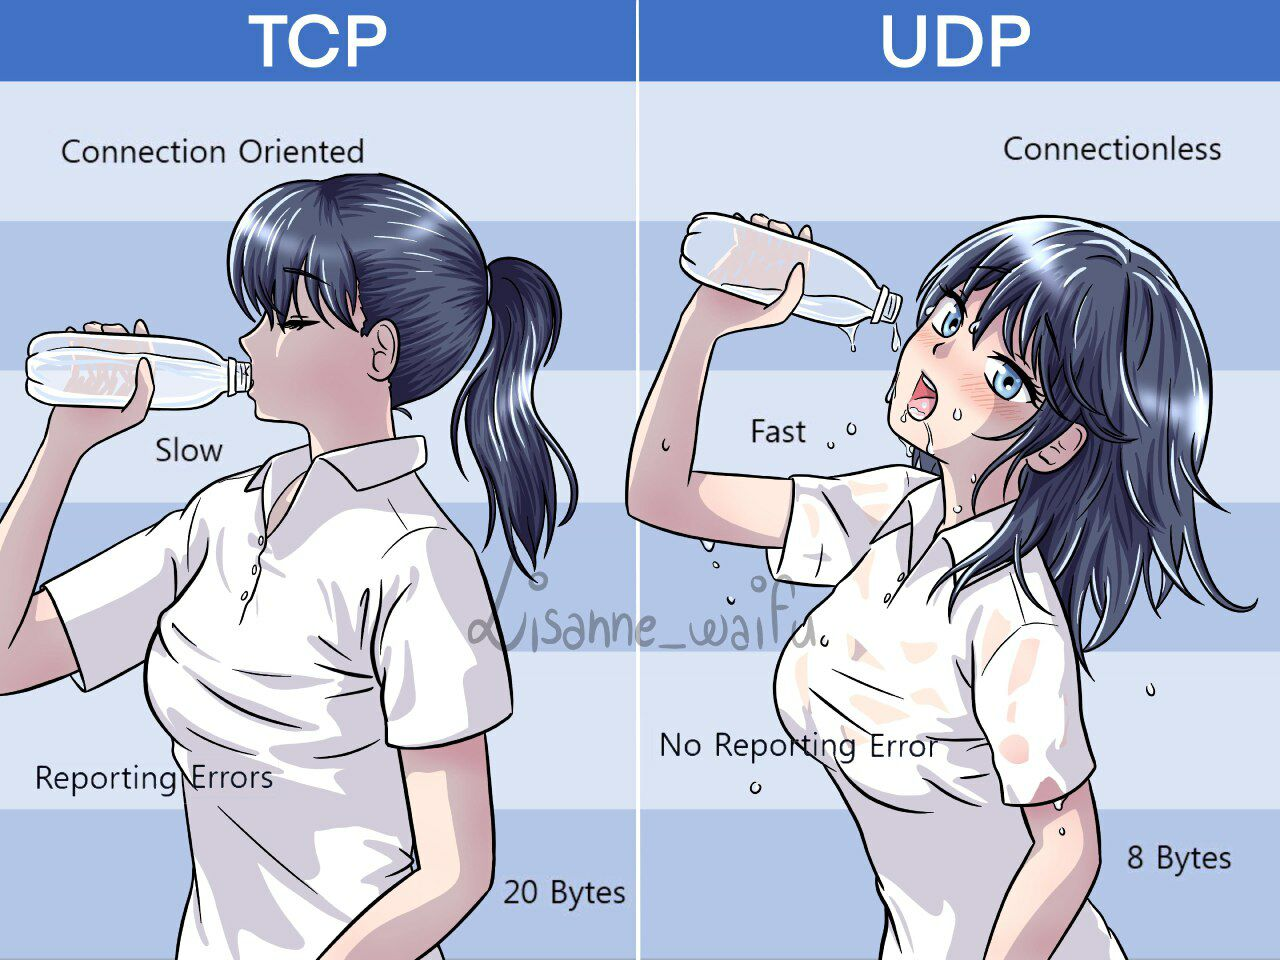
\includegraphics[scale = 0.13]{images/TCP_and_UDP.jpg}
				\caption{TCP与UDP}
			\end{minipage}
			\begin{minipage}{20em}
				\centering
				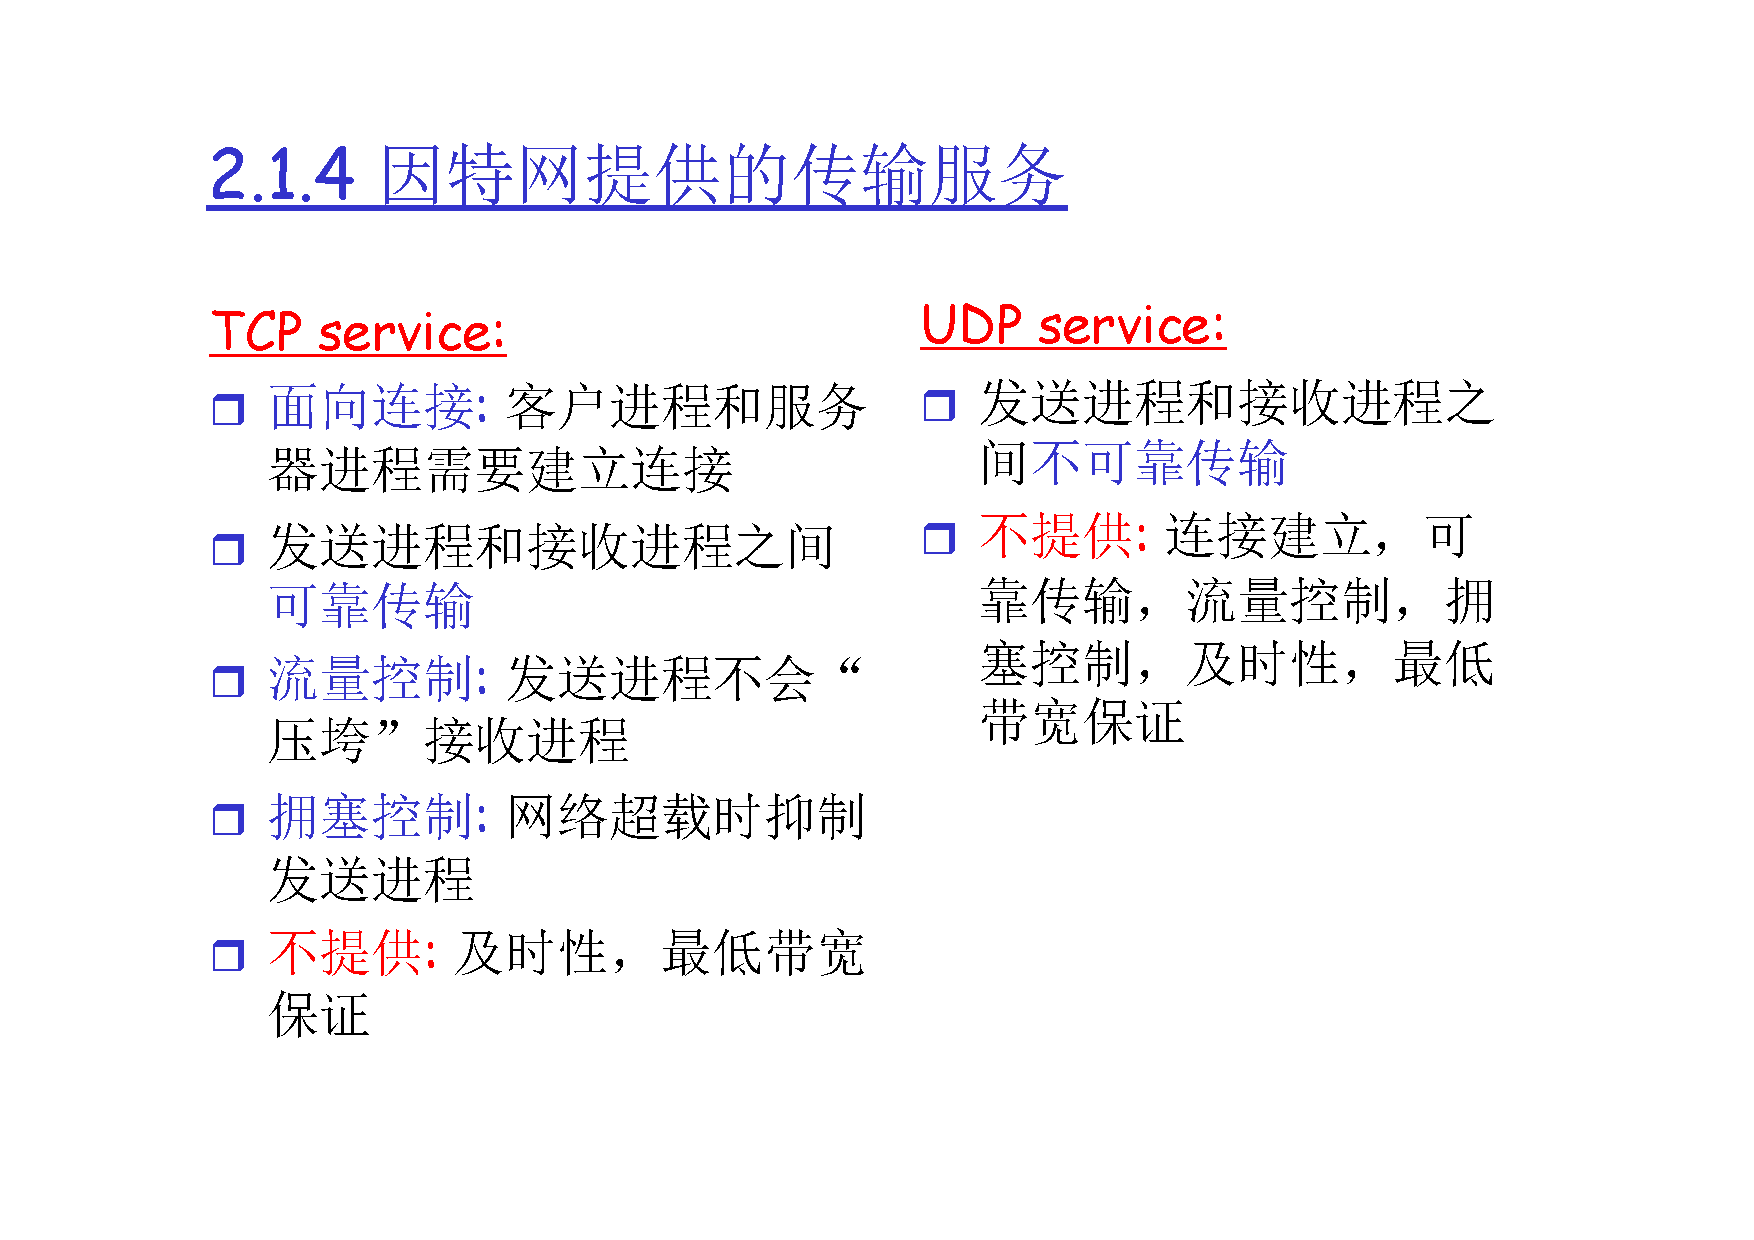
\includegraphics[scale = 0.27]{images/TCP_and_UDP_2.pdf}
				\caption{TCP与UDP}
			\end{minipage}
		\end{figure}
	\section{网络核心}
		电路交换和分组交换\par
		电路交换:为线路预留端到端资源,链路带宽(尤其是瓶颈带宽)决定了通信能力,专用资源不共享,一旦建立起来就可以保证性能,需要建立连接。网络资源(如带宽)被划分成片,可以频分 (FDM)、时分 (TDM)、波分 (WDM)\par
		分组交换:存储-转发(分组每次移动是一跳),在转发之前,结点必须收到整个分组\par
		分组交换可以提升网络的容量:假设线路是1Mbps,每个用户在活跃的时候用掉100kbps,有10\%的时间是活跃的。若使用分组交换,则$\ge10$个用户活跃的概率,由二项分布可得为\[1-\sum_{n=0}^9{35\choose n}p^n(1-p)^{35-n}\]
	\section{分组交换中的时延、丢包和吞吐量}
		分组延迟的来源有四:结点处理延迟、排队延迟、传输延迟、传播延迟。传输延迟是指将分组发送到链路上的时间。
		\[d_{nodel}=d_{proc}+d_{queue}+d_{trans}+d_{prop}\]\par
	\section{协议层次和服务类型}
		\subsection{服务和服务访问点}
		\begin{enumerate}
			\item 服务(Service):低层实体向上层实体提供它们之间的通信的能力
			\begin{enumerate}
				\item 服务用户(service user)
				\item 服务提供者(service provider)
			\end{enumerate}
			\item 原语(primitive):上层使用下层服务的形式,高层使用低层提供的服务,以及低层向高层提供服务都是通过服务访问原语来进行交互的
			\item 服务访问点 SAP (Services Access Point) :上层使用下层提供的服务通过层间的接口
			\begin{enumerate}
				\item 例子:邮箱
				\item 地址(address):下层的一个实体支撑着上层的多个实体,SAP有
				标志不同上层实体的作用
				\item 可以有不同的实现,队列
				\item 例子:传输层的SAP:端口(port)
			\end{enumerate}
		\end{enumerate}
		\subsection{服务和协议}
		\begin{enumerate}
			\item 服务与协议的区别
			\begin{enumerate}
				\item 服务(Service):低层实体向上层实体提供它们之间的通信的能力,是通过原语(primitive)来操作的,垂直
				\item 协议(protocol):对等层实体(peer entity)之间在相互通信的过程中,需要遵循的规则的集合,水平
			\end{enumerate}
			\item 服务与协议的联系
			\begin{enumerate}
				\item 本层协议的实现要靠下层提供的服务来实现
				\item 本层实体通过协议为上层提供更高级的服务
			\end{enumerate}
		\end{enumerate}

	\chapter{应用层}
	\section{应用层协议原理}
		\subsection{网络应用架构}
		网络核心中没有应用层功能,网络应用只在端系统上存在,快速网络应用开发和部署。应用层可能的应用架构:客户-服务器模式(C/S),或者对等模式(P2P),或者混合体
		\paragraph{客户-服务器模式}
		服务器:一直运行,并有固定的IP和周知的端口号;客户机:与互联网有间歇性的连接,可能是动态IP地址,不直接与其它客户端通信
		\paragraph{对等体体系结构}
		每一个节点既是客户端又是服务器;自扩展性——新peer节点带来新的服务能力,当然也带来新的服务请求;参与的主机间歇性连接且可以改变IP地址;难以管理
		\subsection{进程通信}
		不同主机上的进程通过交换报文进行通信。对每对通信进程,我们通常将这两个进程之一标识为客户,另一个标识为服务器。其各自的定义如下:
		\begin{quote}
			\textit{在一对进程之间的通信会话场景中,发起通信(即在该回话开始时发起与其他进程的联系)的进程被标识为客户,在回话开始时等待联系的是服务器}
		\end{quote}
		进程编址需要IP地址和端口号
		\subsection{因特网提供的运输服务}
		因特网(更一般的是TCP/IP网络)为应用程序提供了两个运输协议,即UDP和TCP。
		\paragraph{TCP Service}
		TCP服务模型包括面向连接服务和可靠数据传输服务。TCP链接是全双工的,即连接双方的进程可以在此链接上同时进行报文收发,当应用程序结束发送时,需要拆除该链接。TCP还有拥塞控制机制
	\section{Web和HTTP}
		\subsection{HTTP概况}
		web页面是由对象组成的。对象可以是HTML文件、JPEG图像、Java小程序、声 音剪辑文件等。Web页含有一个基本的HTML文件,该基本HTML文 件又包含若干对象的引用(链接)。通过URL对每个对象进行引用。访问协议,用户名,口令字,端口等。\par
		HTTP是无状态的,即服务器不保存有关客户请求的任何有关信息
		\subsection{非持续链接和持续链接}
		非持久连接在一个TCP连接上最多传输一个对象,持续连接可以发送多个对象。又由于持续连接可以采用流水,效率会更高\par
		关于响应时间模型:往返时间RTT:一个小的分组从客户端到服务器,在回到客户端的时间(传输时间忽略)。响应时间是2RTT+传输时间(握手+请求和响应)
		\subsection{HTTP报文格式}
		\subsection{用户-服务器状态:cookies}
		cookies是在\textit{用户端}系统中维护的,由用户的浏览器管理
	\section{FTP}
		FTP使用了两个端口
		\begin{figure}[h!]
			\centering
			\begin{minipage}{20em}
				\centering
				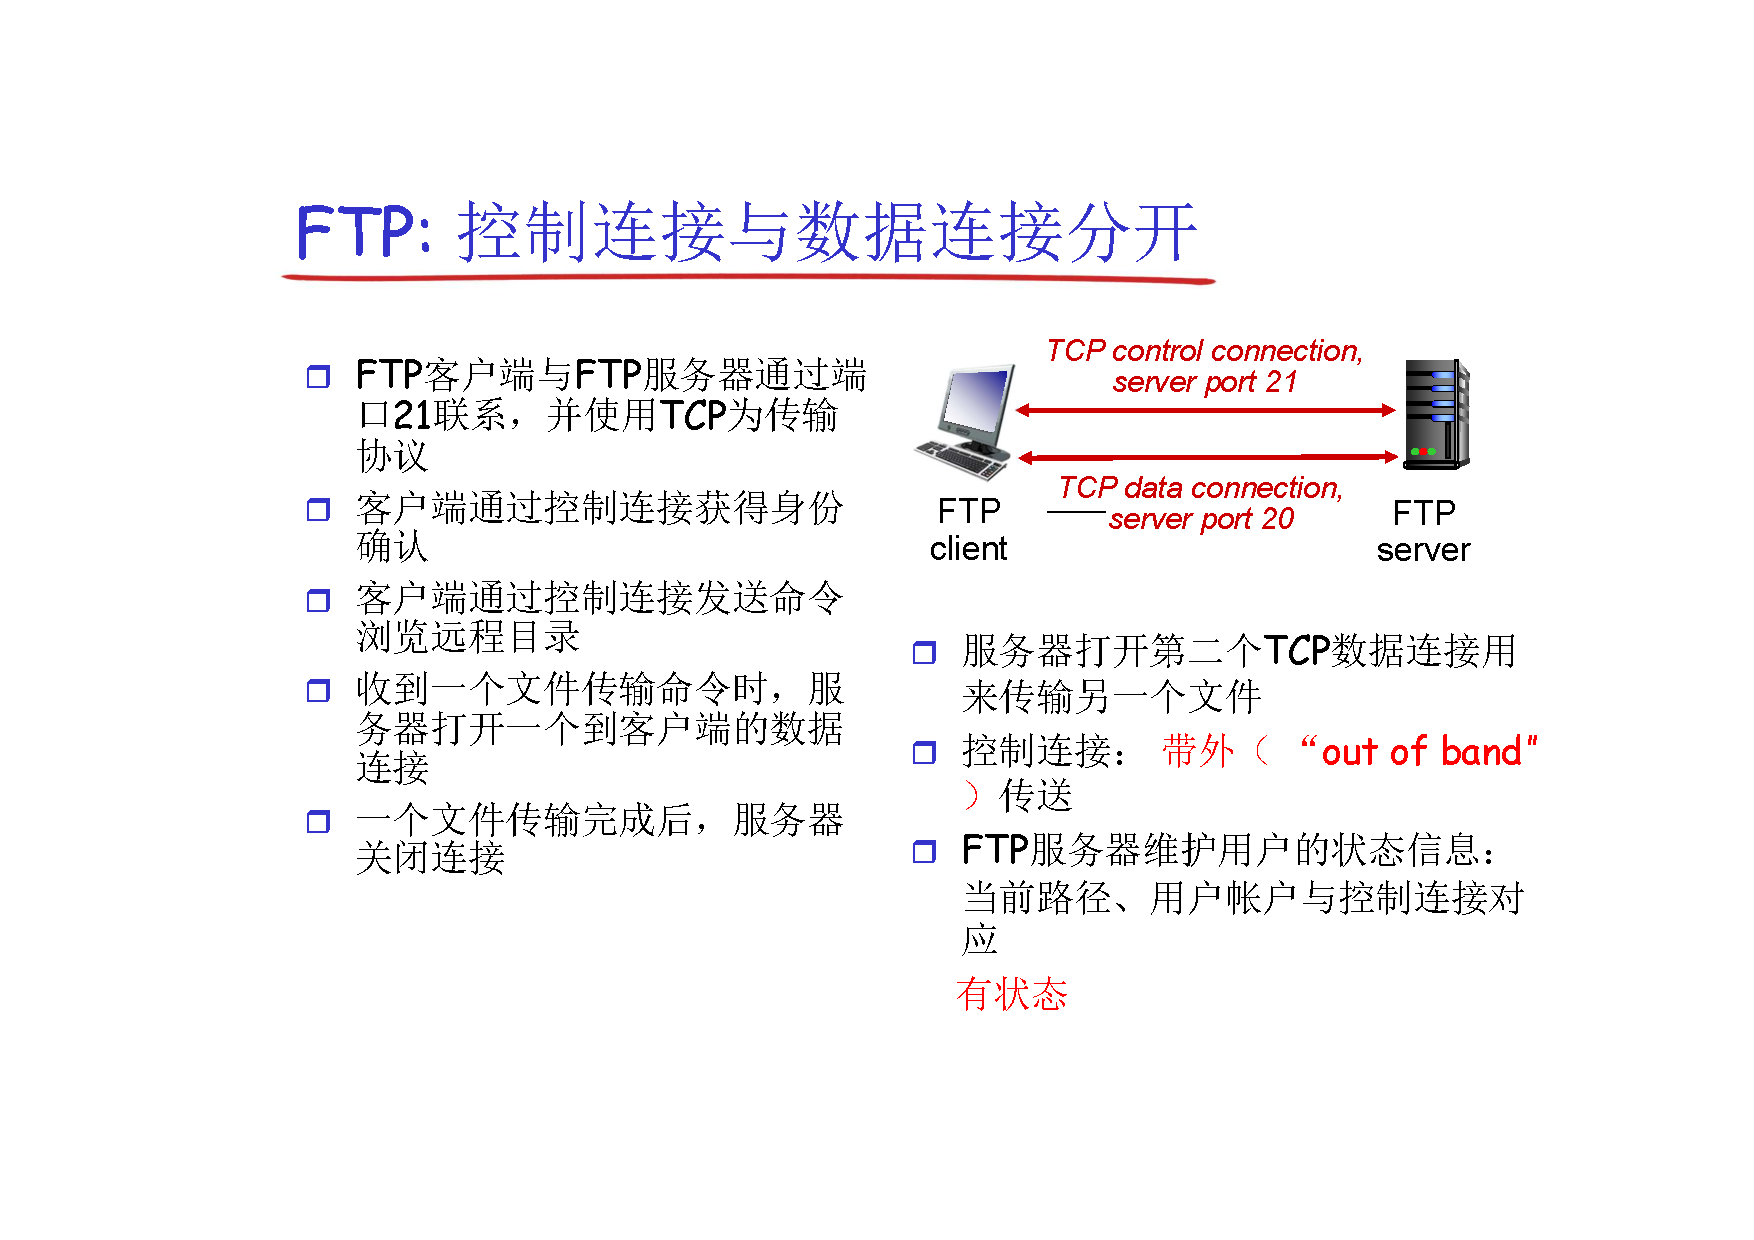
\includegraphics[scale = 0.3]{images/FTP_2_ports_1.pdf}
			\end{minipage}
			\begin{minipage}{20em}
				\centering
				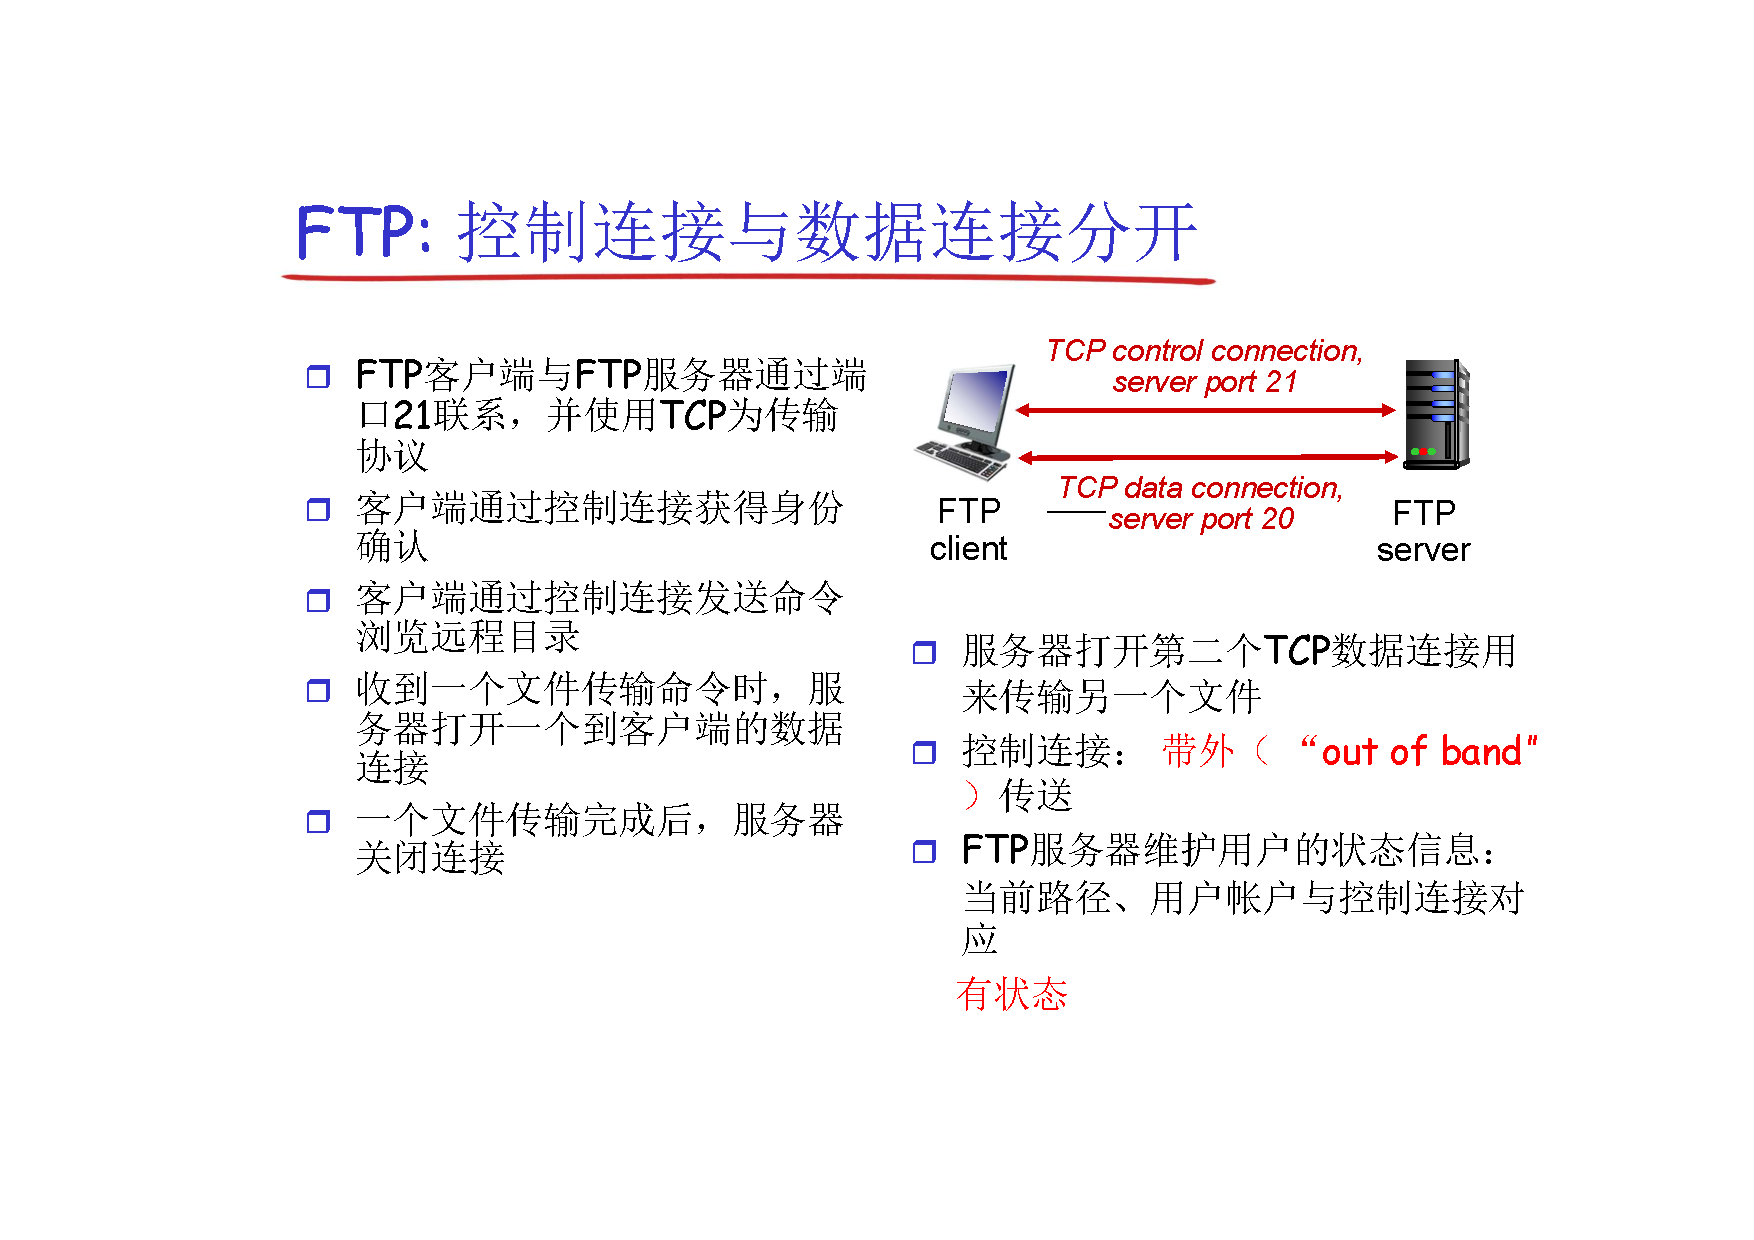
\includegraphics[scale = 0.3]{images/FTP_2_ports_1.pdf}
			\end{minipage}
		\end{figure}
	\section{Email}
		SMTP和HTTP挺像的,总结如下:\par
		\begin{figure}[h!]
			\centering
			\begin{minipage}{40em}
				\centering
				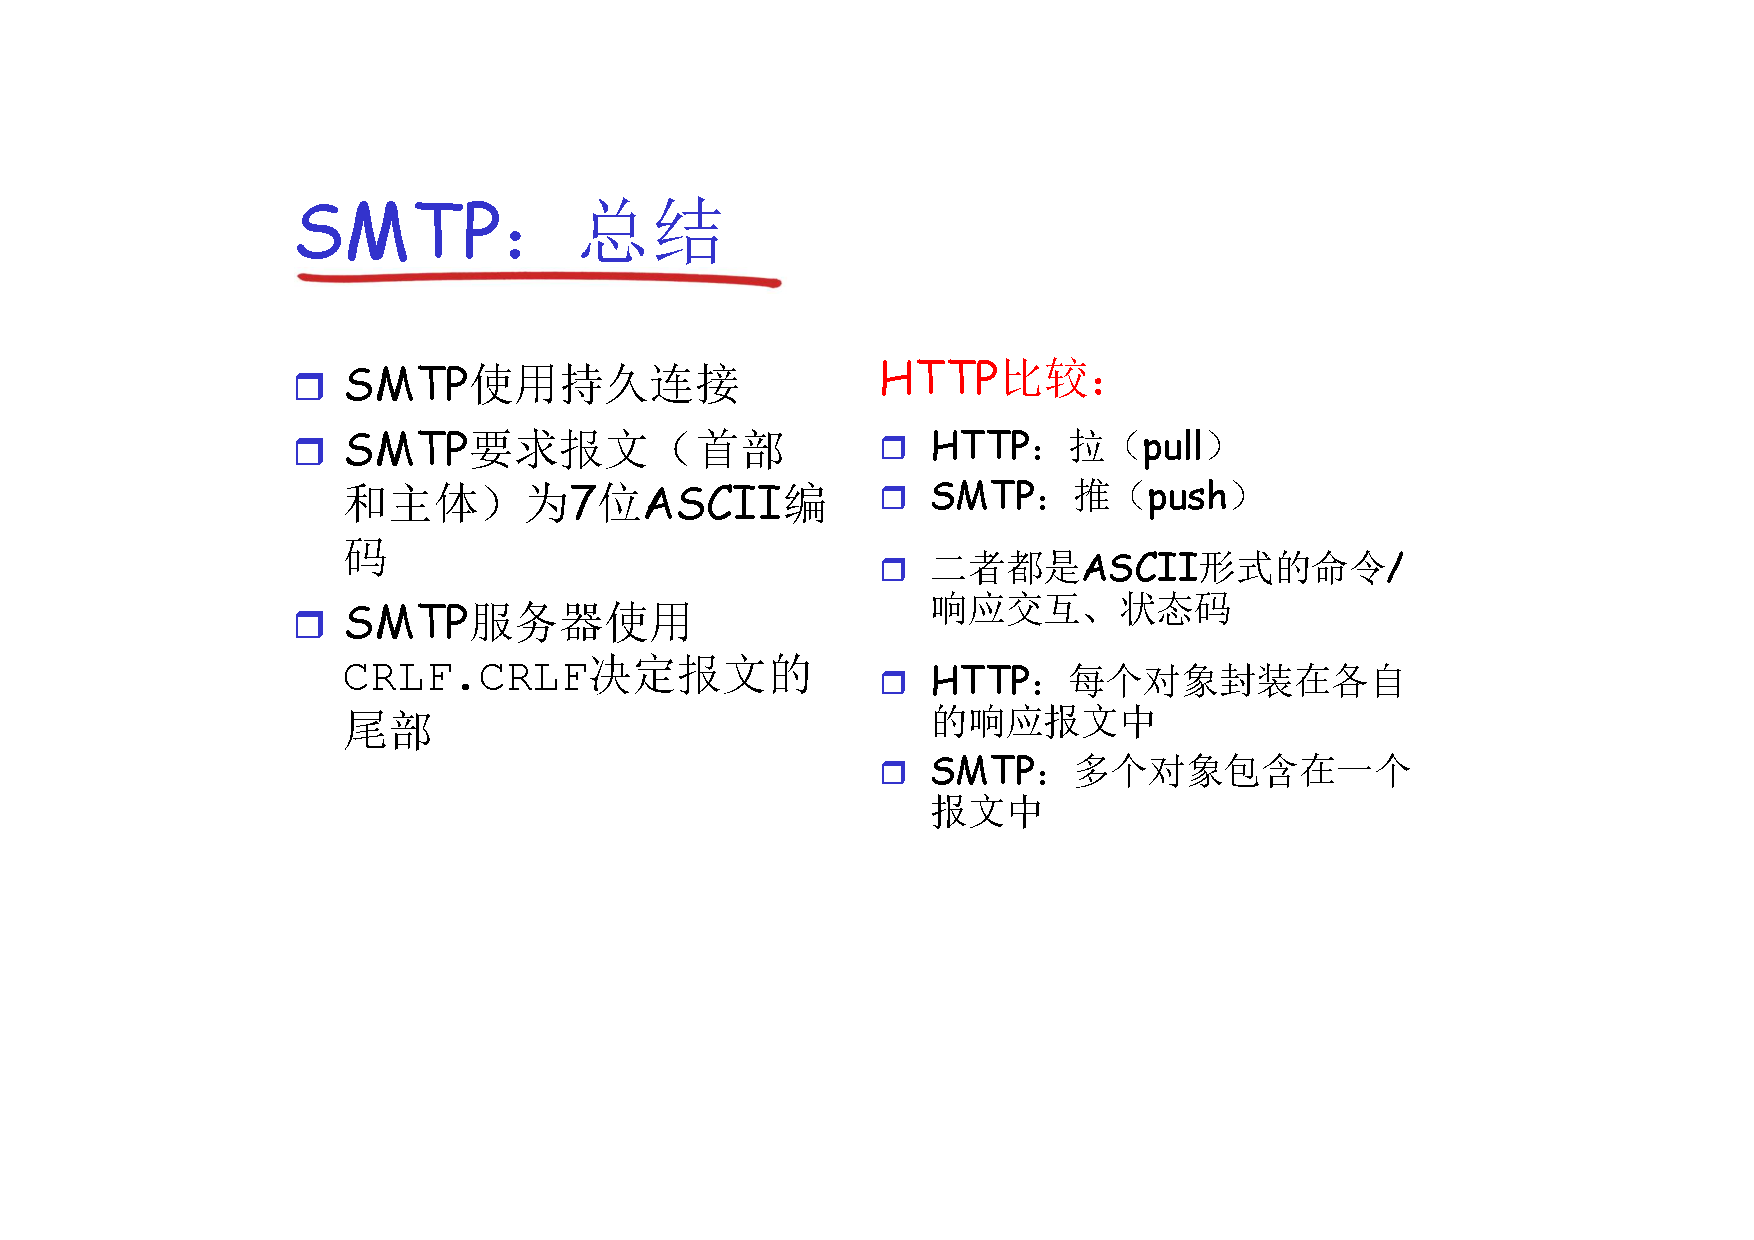
\includegraphics[scale = 0.5]{images/SMTP_and_HTTP.pdf}
			\end{minipage}
		\end{figure}\par
		其中拉协议指,在方便的时候,某些人在web服务器上装载信息,用户使用HTTP从该服务器拉取这些信息。特别是TCP连接是由想接收文件的机器发起的。而推协议,指发送邮件服务器把文件推向接收邮件服务器。特别是TCP连接是由要发送文件的机器发起的。\par
		值得注意的是,SMTP要求每个报文(\textbf{包括他们的体})采用7bit ASCII码格式。如果包含了非7bit ASCII字符(如具有重音的法文字符)或二进制数据(如图形文件),则必须按照 7bit ASCII进行编码
	\section{DNS}
	\section{P2P应用}
	\section{CDN}
	\section{TCP socket 编程}
	\section{UDP socket 编程}

	\chapter{运输层}
	\section{概述和运输层服务}
		在应用程序看来,运输层(PPT为\textit{传输层})为运行在不同主机上的应用进程提供了进程间的逻辑通信。从应用程序的位置来看,通过逻辑通信,运行不同进程的主机好像直接相连一样;实际上,这些主机也许位于地球的两侧通过很多路由器和多种不同类型的链路相连。同应用层一样,运输层也是只有运行在端系统上的。在发送方,将应用层的报文(拆分)并封装为报文段;在接收方做逆处理,从收到的报文段中取出载荷,重组为报文。\par
		网络层服务是主机间的\textit{逻辑}通信,而运输层是进程间的逻辑通信,它依赖于网络层的服务(继承带宽、延迟的限制)并对网络层的服务进行增强(解决数据丢失、顺序混乱,并加密)。有些服务是可以加强的:不可靠$\to$可靠、安全。但有些服务是不可以被加强的:带宽,延迟\par
		类比:两个家庭的通信(Ann家的12个小孩给另Bill家的12个小孩发信)
		\begin{enumerate}
			\item 主机:家庭
			\item 进程:小孩
			\item 应用层报文:信封中的信件(可以类比信封为包装的报文段附加的部分)
			\item 传输协议:Ann 和 Bill(为家庭小孩提供复用解复用服务)
			\item 网络层协议:邮政服务(家庭-家庭的邮包传输服务)
		\end{enumerate}
		在本书中,我们将TCP和UDP的分组统称为\textit{报文段},而将\textit{数据报}名称留给网络层分组。\par
		TCP和UDP最基本的责任是,将两个端系统间IP的交付服务扩展为运行在端系统上的两个进程之间的交付服务。将主机间交付扩展到进程间交付被称为运输层的多路复用与多路分解(transport-layer multiplexing and demultiplexing)。TCP力求为每一个通过一条拥塞网络链路的连接平等地共享网络链路带宽。
	\section{多路复用与解复用}
		\begin{enumerate}
			\item 在发送方主机多路复用:从多个套接字接收来自多个进程的报文,根据套接字对应的IP地址和端口号等信息对报文段用头部加以封装(该头部信息用于以后的解复用)
			\item 在接收方主机多路解复用:根据报文段的头部信息中的IP地址和端口号将接收到的报文段发给正确的套接字(和对应的应用进程)
		\end{enumerate}
		为了将报文交给正确的套接字
		\begin{enumerate}
			\item 主机中每个套接字应分配一个唯一的标识
			\item 报文段中有特殊字段指示要交付的套接字
			\item 发送方传输层需在报文段中包含目的套接字标识(多路复用)
			\item 接收方传输层需将报文段中的目的套接字标识与本地套接字标识进行匹配,将报文段交付到正确的套接字(多路分解)
		\end{enumerate}
		回忆一下2.7节,一个进程(作为网络应用的一部分)有一个或多个套接字,它们相当于在网络和进程之间传递数据的门户
		\begin{figure}[h!]
			\centering
			\begin{minipage}{40em}
				\centering
				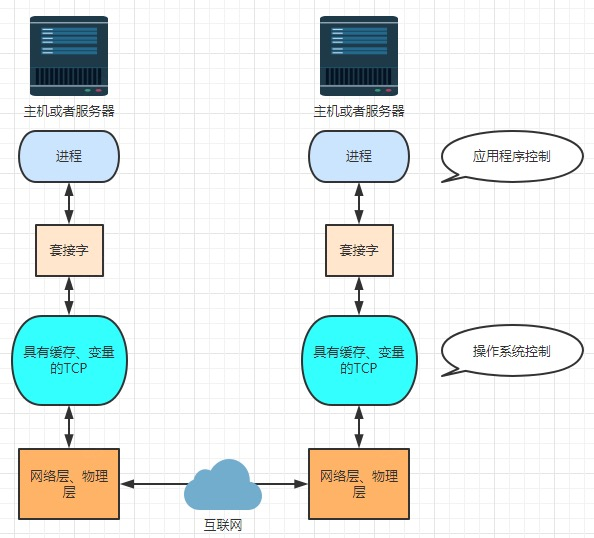
\includegraphics[scale = 0.4]{images/Progress_Socket_and_TCP.jpg}
				\caption{应用进程、套接字、运输层}
			\end{minipage}
		\end{figure}
		端口号是socket标识的重要组成部分,是一个16位的二进制数,其中0~1023作为保留端口号给公共域协议使用,称众所周知的端口号。一般实现公共域协议的服务器会绑定到这个区域内。在主机上的每一个套接字都能够分配到一个端口号,当接收方传输层接收到一个UDP报文时,检查其中的目标端口号,并将这个报文交付到具有该端口号的套接字。\par
		值得注意的是,在多路解复用的过程中,UDP的socket选择标识为报文段中的二元组(目的IP,目标端口号),而TCP用的标识是(源IP,源PORT,目标IP,目标PORT)的四元组。所以对于UDP,具备相同目标IP地址和目标端口号,即使是源IP地址或/且源端口号不同的IP数据报,也会被传到相同的目标UDP套接字上。而对于TCP,服务器能够在一个TCP端口上同时支持多个TCP套接字:每个套接字由其四元组标识(有不同的源IP和源PORT)。比如Web服务器对每个连接客户端有不同的套接字(非持久对每个请求有不同的套接字)。
		\begin{figure}[h!]
			\centering
			\begin{minipage}{40em}
				\centering
				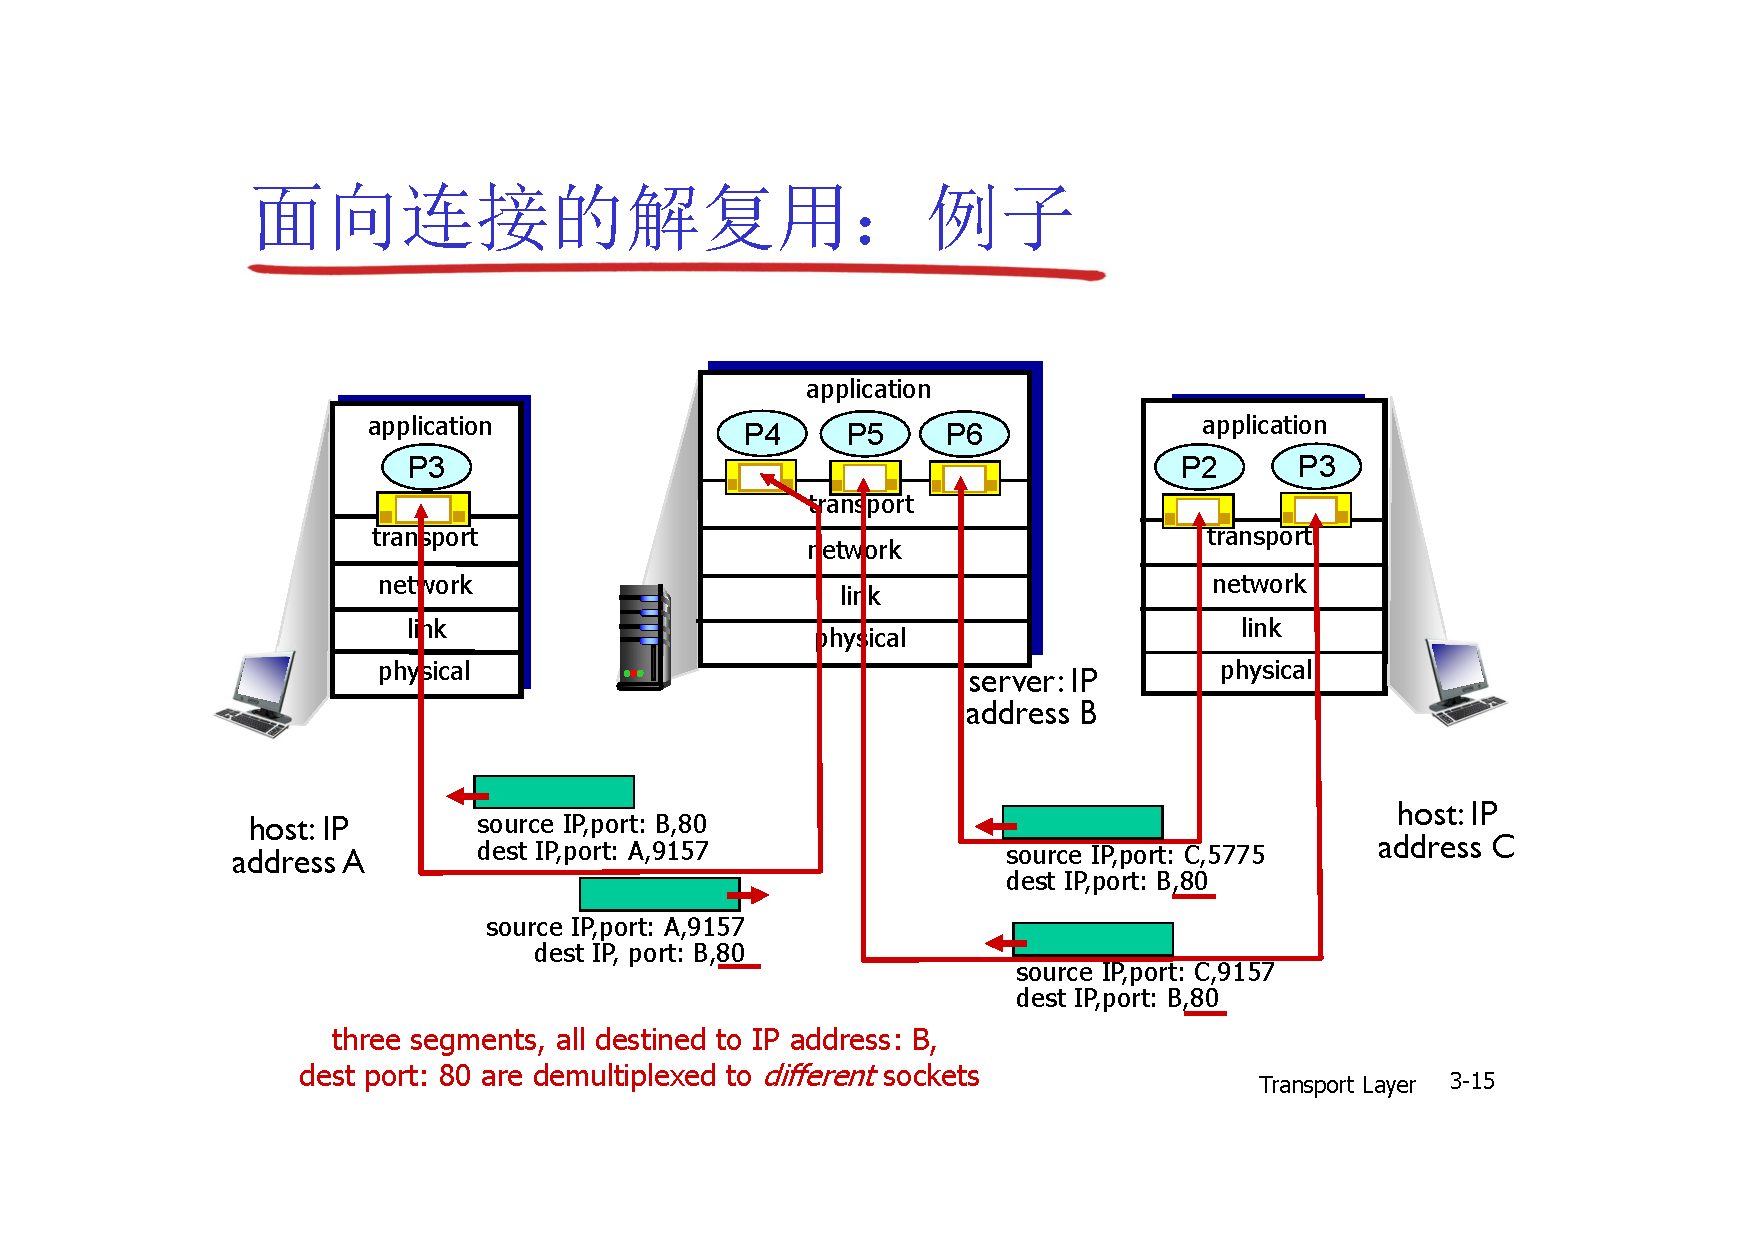
\includegraphics[scale = 0.4]{images/TCP_Socket_Ports.pdf}
			\end{minipage}
		\end{figure}
		在上图的实际实现中,有一个初始的socket,每接收到一个对应到本PORT的连接请求就“fork”出来一个新的socket来相应
	\section{无连接传输:UDP}
		UDP即用户数据报协议,其报文结构为源端口号、目的端口号、长度、检验和(奇偶校验)应用数据(报文)。对于UDP检验和的确定,其规则\href{https://www.zhihu.com/question/66620337}{如下}:UDP校验和就是二进制反码求和(先求和然后再求反码),但在求和过程中假如首位溢出需要进位,需要\textbf{回卷},即把前面多出去的1加到最后。比如下面这个例子:\par
		两组数据分别为1001和1111,则求和时,由于首位溢出需要回卷,则为:
		\[\begin{aligned}
			1001&\\
			1111&\\
			1&\\
			----&\\
			1001&
		\end{aligned}\]\par
		取反码得到校验和为$0110$。在接收端进行校验时,将校验范围与校验和相加,若为0xFFFF则通过校验
	\section{可靠数据传输的原理}
		可靠数据传输(rdt, reliable data transfer)在应用层、传输层、数据链路层都很重要。可靠数据传输命题大致如下图所示:
		\begin{figure}[h!]
			\centering
			\begin{minipage}{40em}
				\centering
				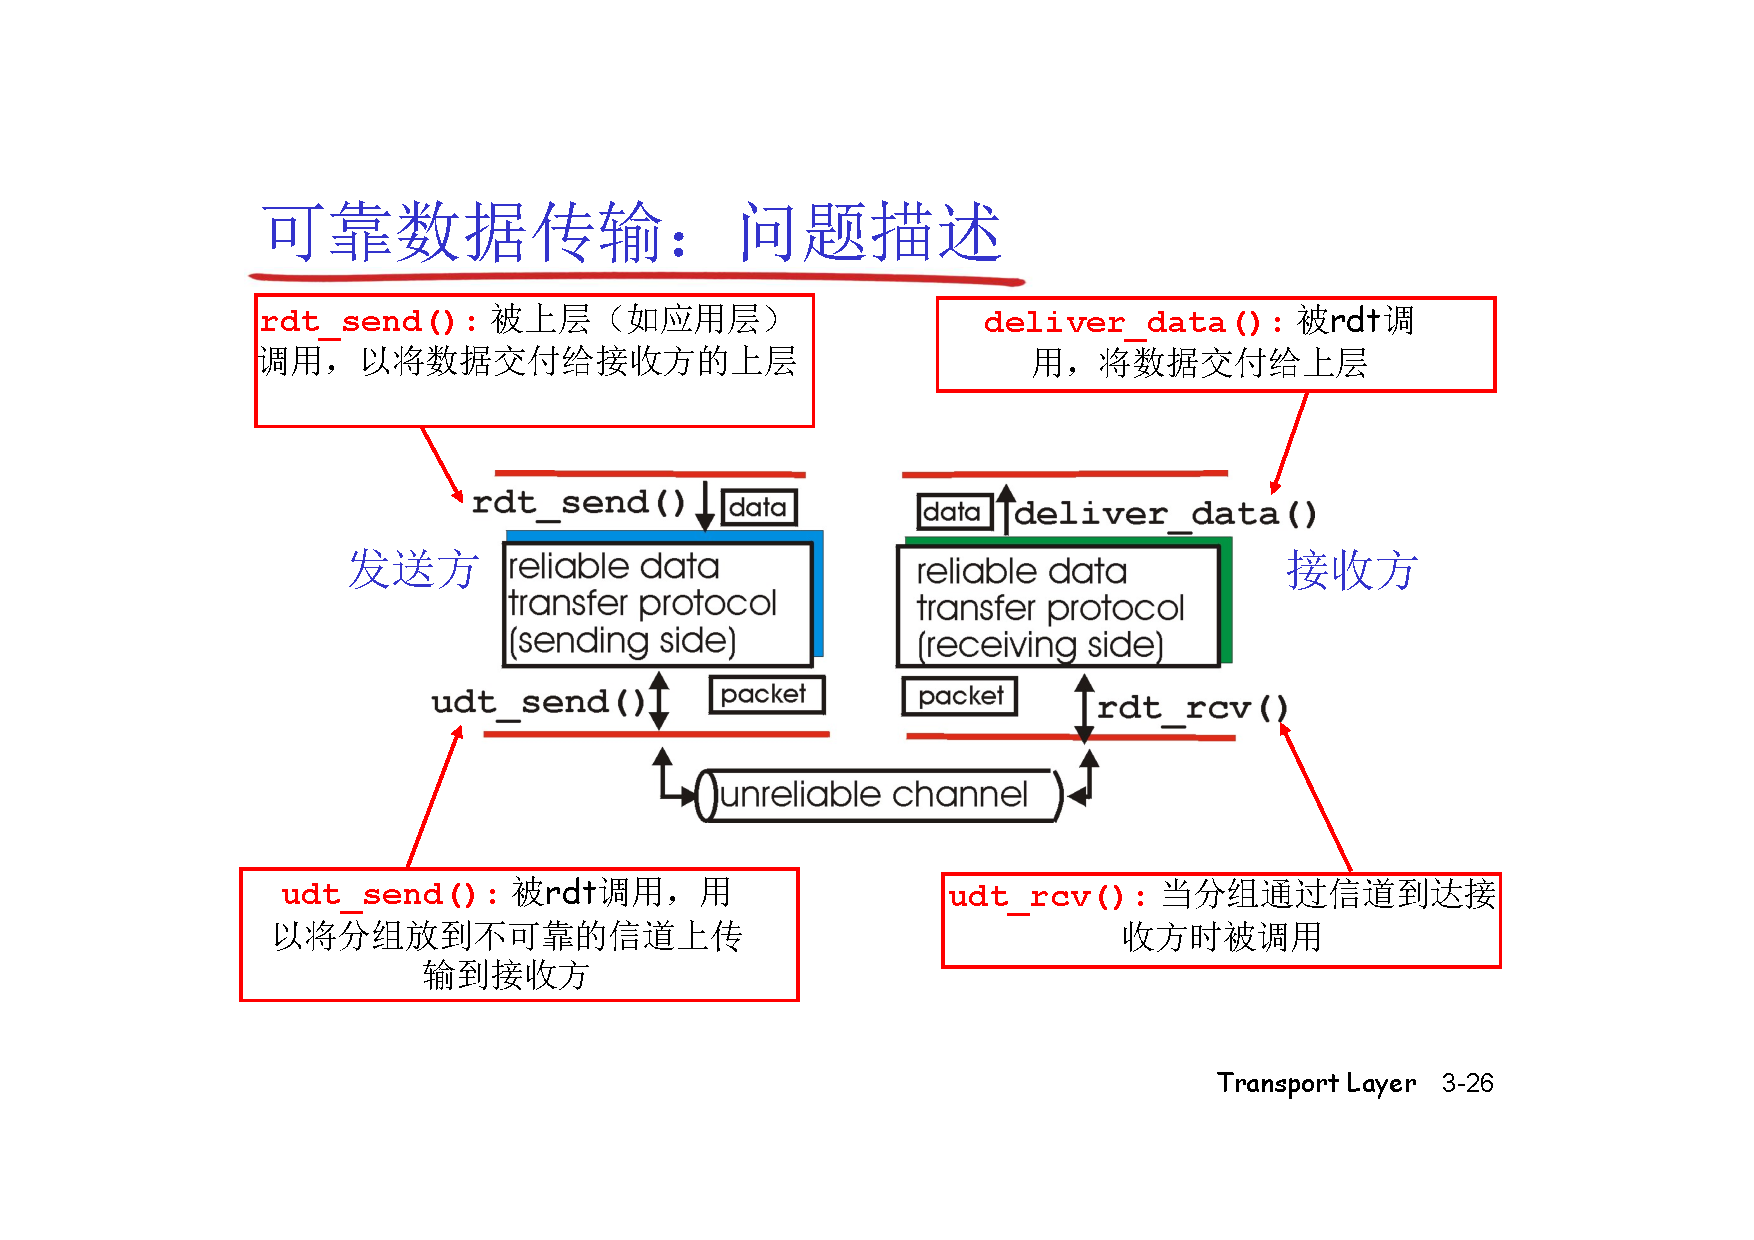
\includegraphics[scale = 0.4]{images/RDT_and_Unreliable_Channel.pdf}
			\end{minipage}
			\begin{minipage}{40em}
				\centering
				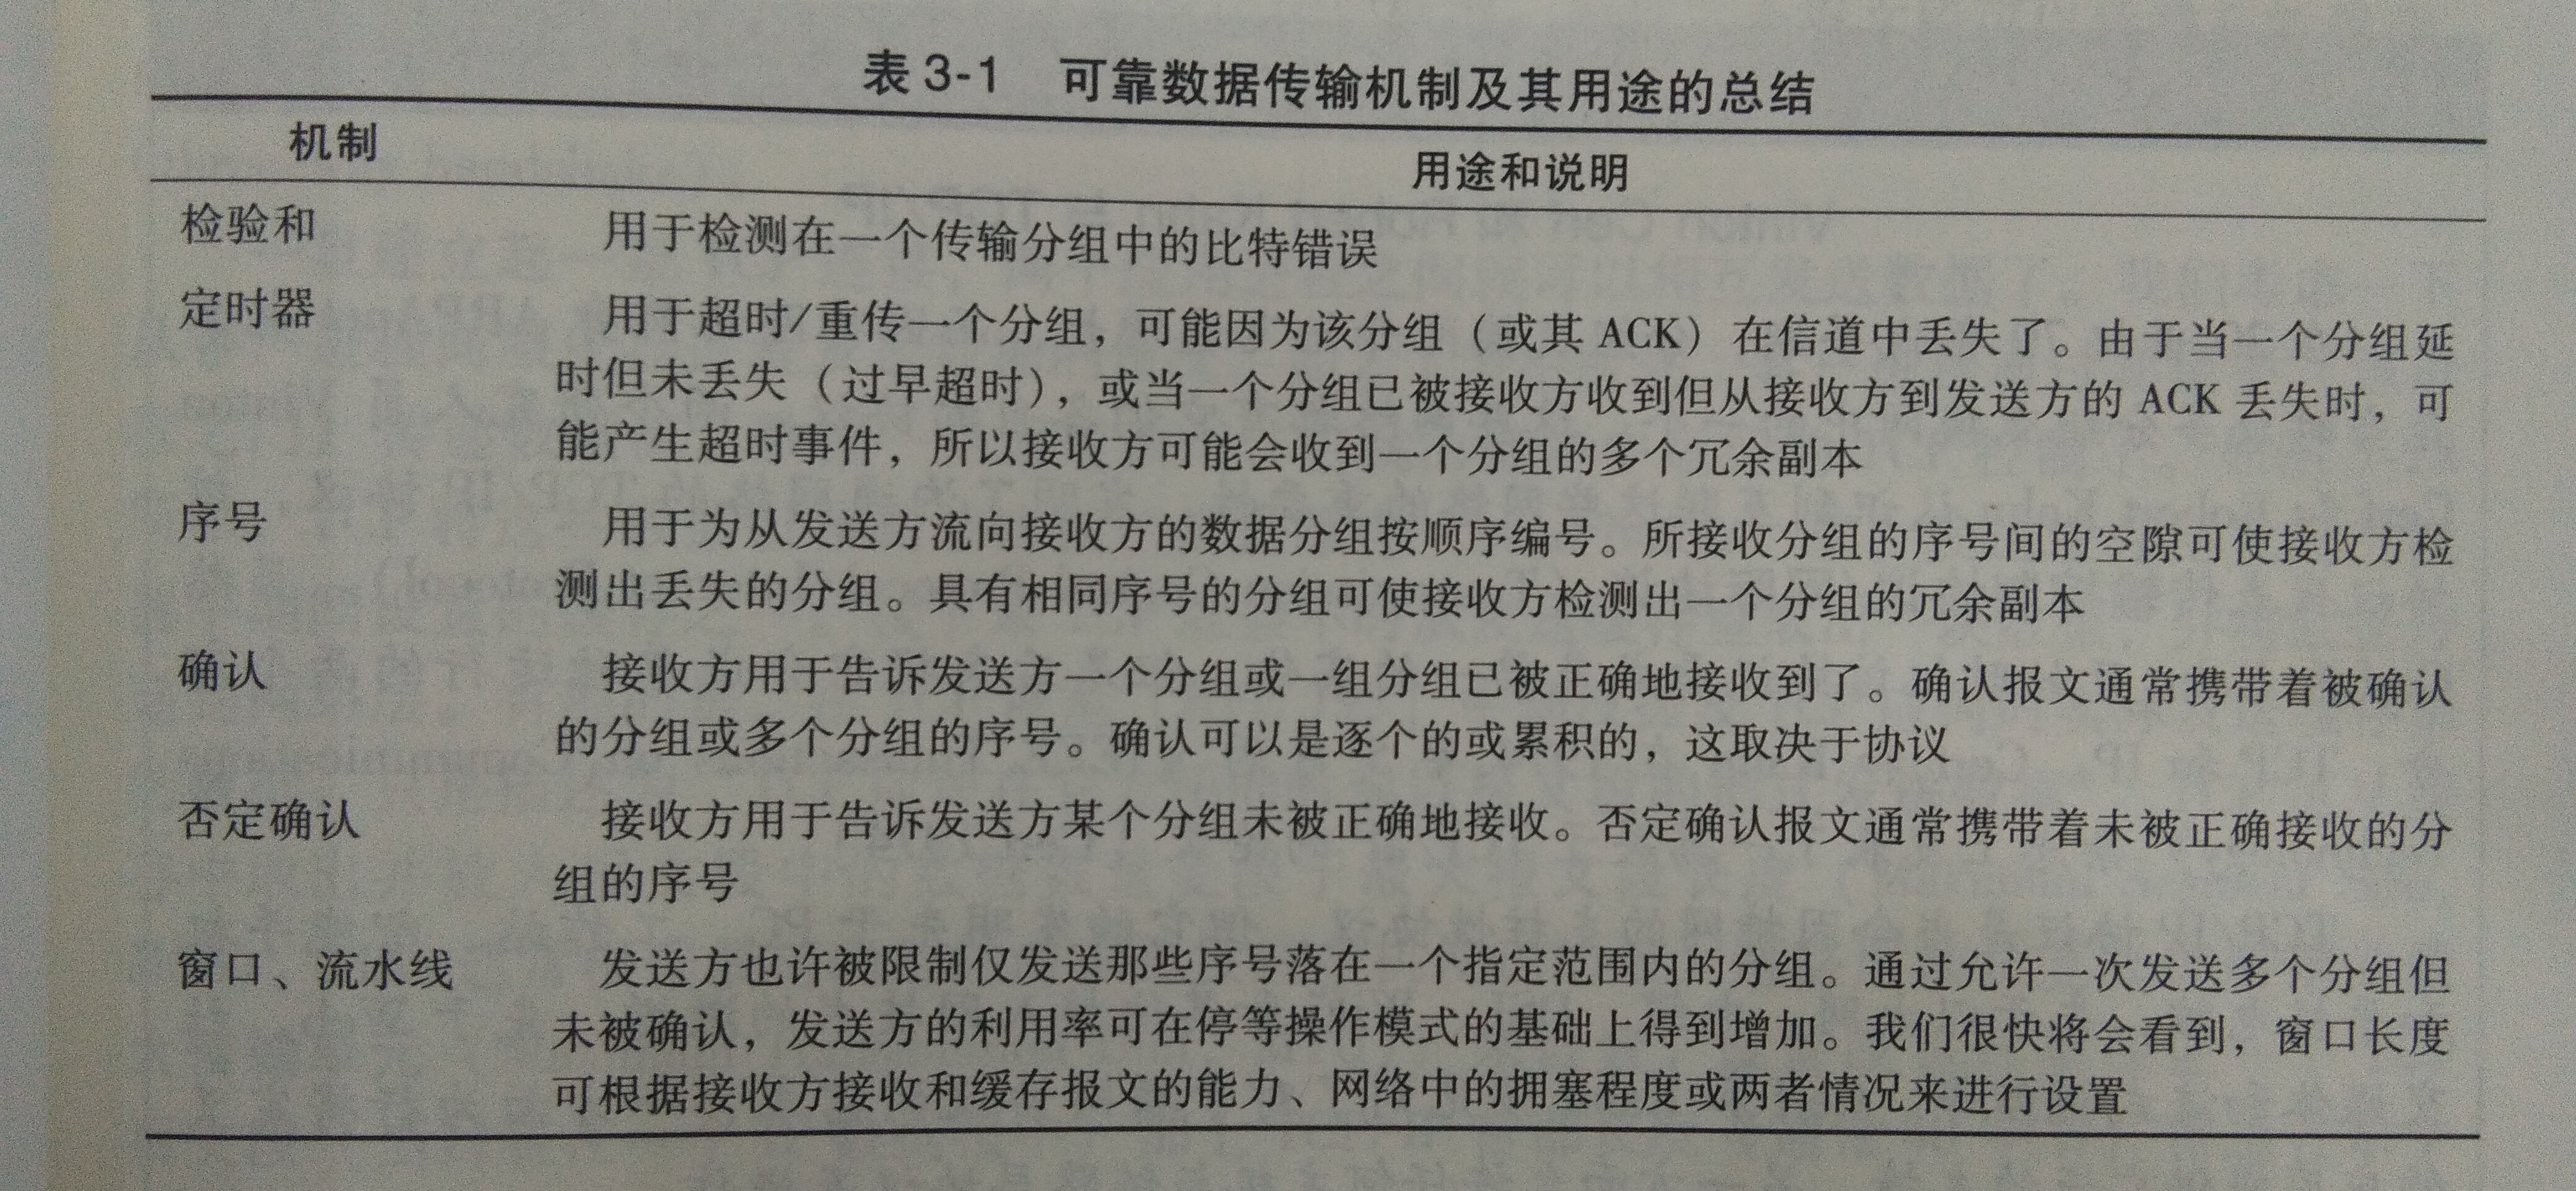
\includegraphics[scale = 0.1]{images/KeKaoShuJuChanShuZongJie.jpg}
			\end{minipage}
		\end{figure}
		\subsection{RDT 1.0:经完全可靠信道的可靠数据传输}
			这是最简单的情形。注意到下列问题是重要的,发送方和接收方有\textbf{各自的}FSM。发送方和接收方各自只有一个状态。\footnote{本书使用的FSM规范:引起变迁的事件先是在表示变迁的横线上方,事件发生时所采取的动作显示在横线下方,如果事件/动作为空,则使用符号$\wedge$,以分别明确地表达缺少动作或事件。初始状态用虚线表示}
			\begin{figure}[h!]
				\centering
				\begin{minipage}{40em}
					\centering
					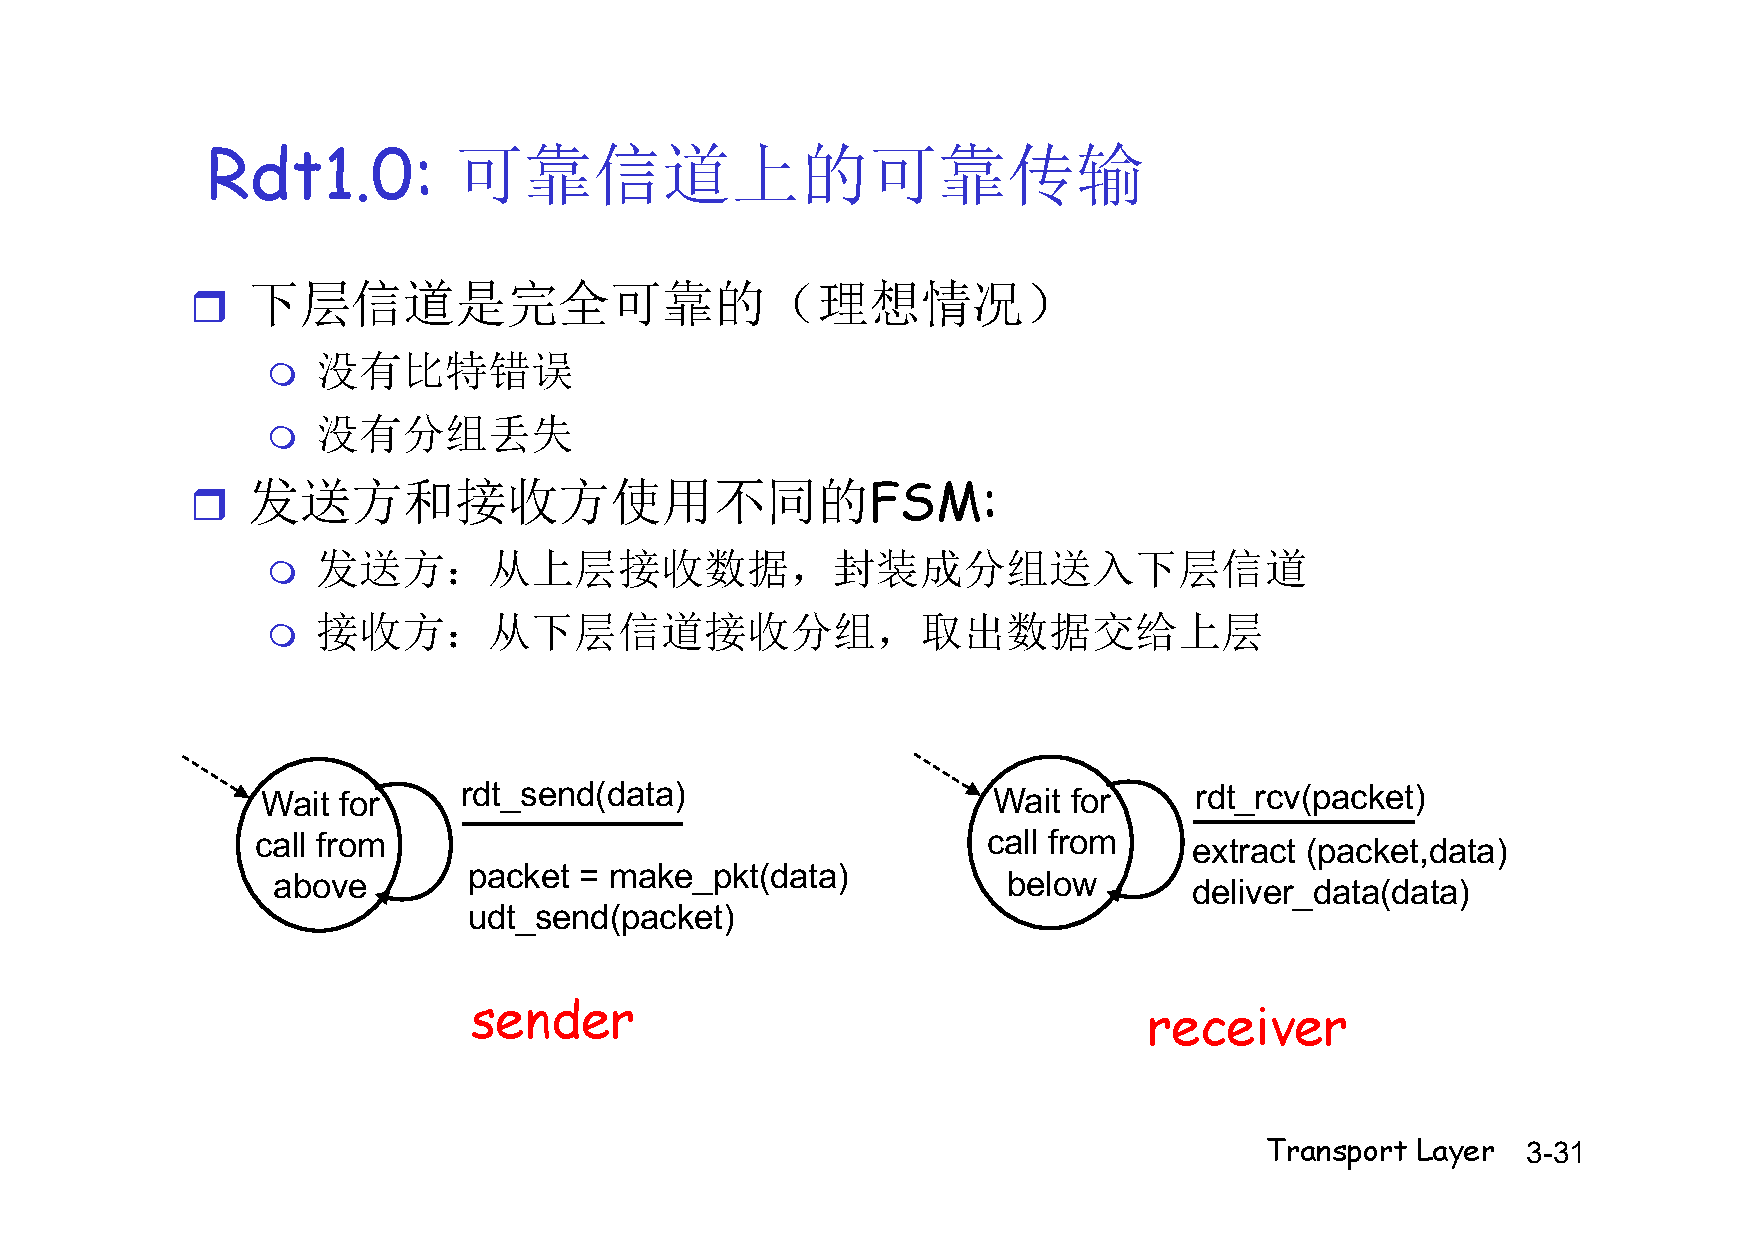
\includegraphics[scale = 0.4]{images/rdt_1_0.pdf}
				\end{minipage}
			\end{figure}
			在这个简单的协议中,\textit{一个单元数据和一个分组没有区别};因为信道完全可靠,接收端不需要反馈信息;由于假定了接收速率和发送速率一样,也不需要限流
		\subsection{RDT 2.0:经具有比特差错信道的可靠数据传输}
			假定顺序不被打乱,但是有些比特可能受损(翻转)。处理此类模型的基本思想是“基于肯定确认和否定确认的重传机制的可靠数据传输协议”,称为自动重传请求协议(Automatic Repeat reQuest, ARQ)。ARQ使用了以下4种机制(书上没写第一个):
			\begin{enumerate}
				\item 发送方差错控制编码、缓存
				\item 差错检测:使用校验码
				\item 接收方反馈:接收方向发送方回送控制报文(“肯定确认”ACK和“否定确认”NAC)
				\item 重传:收到有差错的需要重传
			\end{enumerate}
			\begin{figure}[h!]
				\centering
				\begin{minipage}{40em}
					\centering
					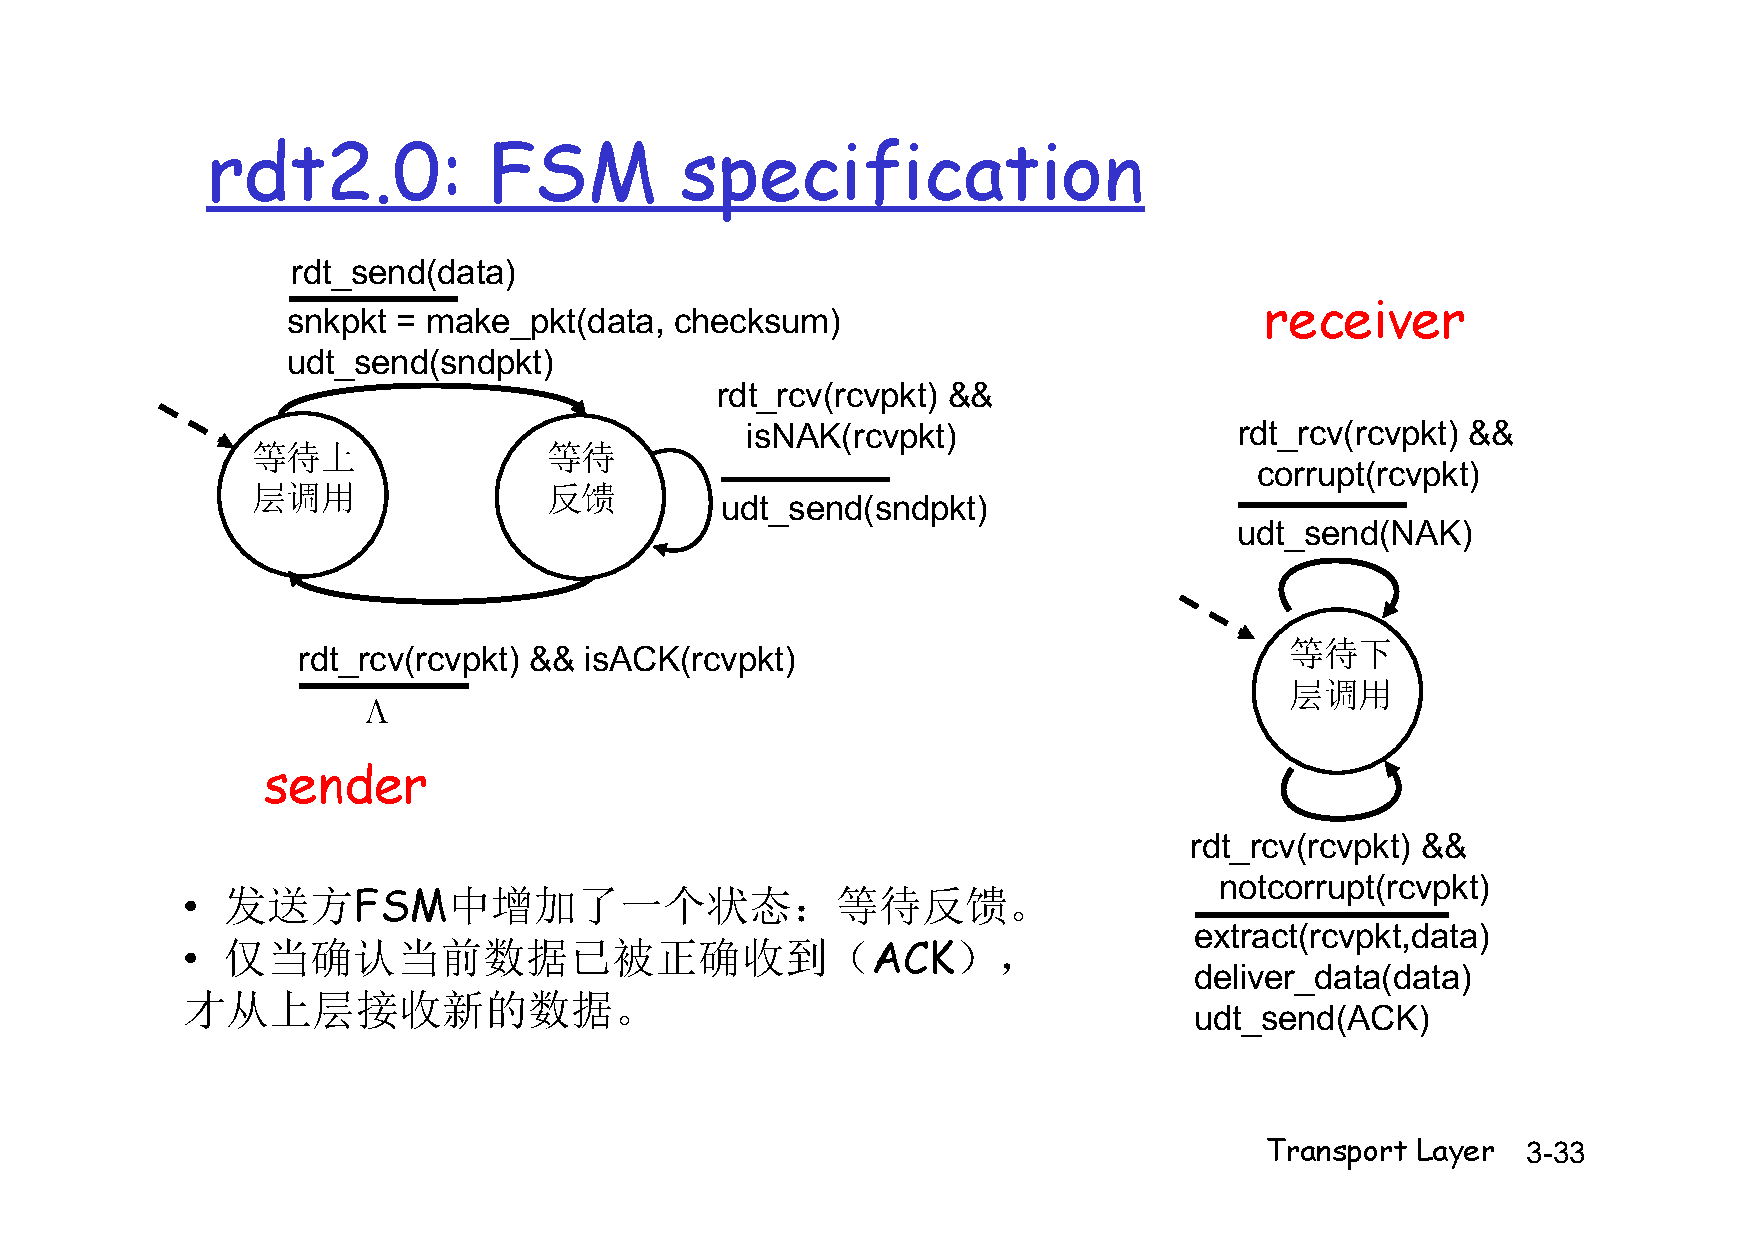
\includegraphics[scale = 0.4]{images/RDT_2_0.pdf}
				\end{minipage}
			\end{figure}
			注意下列事实很重要:当发送方处于等待ACK或NAK的状态时,它\textbf{不能}从上层获得更多的数据。因此rdt2.0这样的协议被称为\textbf{停等}(stop-and-wait)协议
		\subsection{RDT 2.1:发送方处理出错的ACK/NAK}
			rdt2.0有一个fatal flaw,即由于信道的不可靠性,无法保证在反馈信号回送给发送方时,反馈信息分组可以无误到达。所以在除去增加纠错比特位使得接收方可以直接恢复原有信息这种办法以外,还可以采取发送方冗余重传的方式。收到损坏的ACK/NAK分组时,直接重传即可。但是这种方案可能会在接收方造成分组冗余,于是可以在发送分组上加一个序号(标志位),表示是初传还是重传
		\subsection{RDT 2.2:不使用NAK的协议}
			\begin{enumerate}
				\item 接收方
				\begin{enumerate}
					\item 对每一个正确接收的分组发送ACK
					\item ACK中显式携带所确认分组的序号
					\item 若收到出错的分组、或不是期待接收的分组,重发对前一个正确接收分组的ACK
				\end{enumerate}
				\item 发送方:若ACK的序号不是所期待的(表明当前分组未被确认),重发当前分组
				\item 为后面的一次发送多个数据单位做一个准备
				\begin{enumerate}
					\item 一次能够发送多个
					\item 每一个的应答都有:ACK,NACK;麻烦
					\item 使用对前一个数据单位的ACK,代替本数据单位的nak
					\item 确认信息减少一半,协议处理简单
				\end{enumerate}
			\end{enumerate}
		\subsection{RDT 3.0:经具有比特差错和分组丢失的信道的可靠信息传输}
			使用一个倒计时装置,发送方等待ACK一个合理的时间(链路层的timeout时间是确定的,传输层timeout时间是适应式的),到时还没有收到ACK就重传。问题是如果仅仅是延迟了,可能会导致数据冗余。用序列号可以解决,但是接收方在发出ACK时必须指明接收的序列号。因为分组序号在0和1之间交替,因此rdt3.0有时被称为比特交替协议\par
			需要引起注意的是,尽管rdt3.0是一个正确的协议,其停等协议的属性导致了它的性能不佳
		\subsection{流水线可靠数据传输协议}
			参考多周期CPU和流水线CPU的构造,想想为什么会有流水(并行)和如何抛出精确异常(回退N步和选择重传)。为了选择重传,接收方需要设置缓冲区缓存失序的包。\par
			流水线技术对可靠数据传输可以带来如下影响:
			\begin{enumerate}
				\item 必须增加序号范围,因为每一个输送的分组(\textbf{不计算重传的})必须有一个唯一的序号,而且也许由多个在输送中的未确认报文
				\item 协议的发送方和接收方需缓存多个分组。发送方需那些已发送但没有确认的分组(可能重传),接收方需要已经正确接受的分组(可能乱序或者有中间的分组丢失)
				\item 所需序号范围和对缓冲区的要求取决于数据传输协议如何处理丢失、损坏以及延迟过大的分组。
			\end{enumerate}\par
			传输的窗口包括可以发送但还没有发出去的分组,和已经发出去但还没有ACK的分组,也有可能包括已经ACK的分组。他只是要求已发出去但没有被确认的包的数量最多为N,最坏情况下,窗口中的包都是发出去却未收到ACK的。\par
			处理异常主要有两种方法:回退N步(GBN)和选择重传(SR)
		\subsection{回退N步}
			允许发送方发送多个分组而不需要等待确认。GBN的基本思想是,将分组按照一个数组进行放置,一个滑动窗口作为分组的可视范围,那些已被发送但还没有确认的,以及(由于收到ACK而)做好准备发送的分组的许可序号范围。\par
			从另一个角度来看,许可序号是有限的,当一个ACK回到发送方时,就将这个序号传递给下一个没有被分配序号的分组,让他称为“可用,还未发送”状态。这类似于一种流水的折返跑接力赛,假设共有N个接力棒(窗口长度),拿到接力棒的选手进入准备状态(窗口内),这些选手每经过一定的时间就出发,到达终点就返回(ACK),返回之后将接力棒交给正好在窗口之后的分组。\par
			分组序号承载在分组首部的一个固定长度的字段中,TCP有一个32bit的序号字段,不过它是按照字节流进行计数的\par
			GBN的工作原理简单来说,就是
			\begin{enumerate}
				\item 哪里跌倒从哪里站起来:一旦某一个分组传输失败,那后面的都需要重新传输
				\item 最高ACK:接收方仅对正确收到的、序号连续的一系列分组中的最高序号进行确认
				\item 失序复读:若收到失序的分组,丢弃(不在接收端缓存),并重发前一次(或者再之前)的ack分组(已正确收到、序号连续的一系列分组中的最高序号)
				\item 累积确认:若ACK包含序号q,表明“序号至q的分组均正确收到”
				\item 一次性滑动:如果收到序号q的ACK(即使没有收到之前的),整体滑动发送窗口,使基序号= q+1
				\item 超时重传:发送方只对基序号分组使用一个定时器,发送方重传发送窗口中从基序号开始的所有分组
			\end{enumerate}
			计时:GBN在应对超时采用的是维护一个计时器,记录最早的已发送的但还未确认的分组
			\begin{figure}
				\centering
				\begin{minipage}{40em}
					\centering
					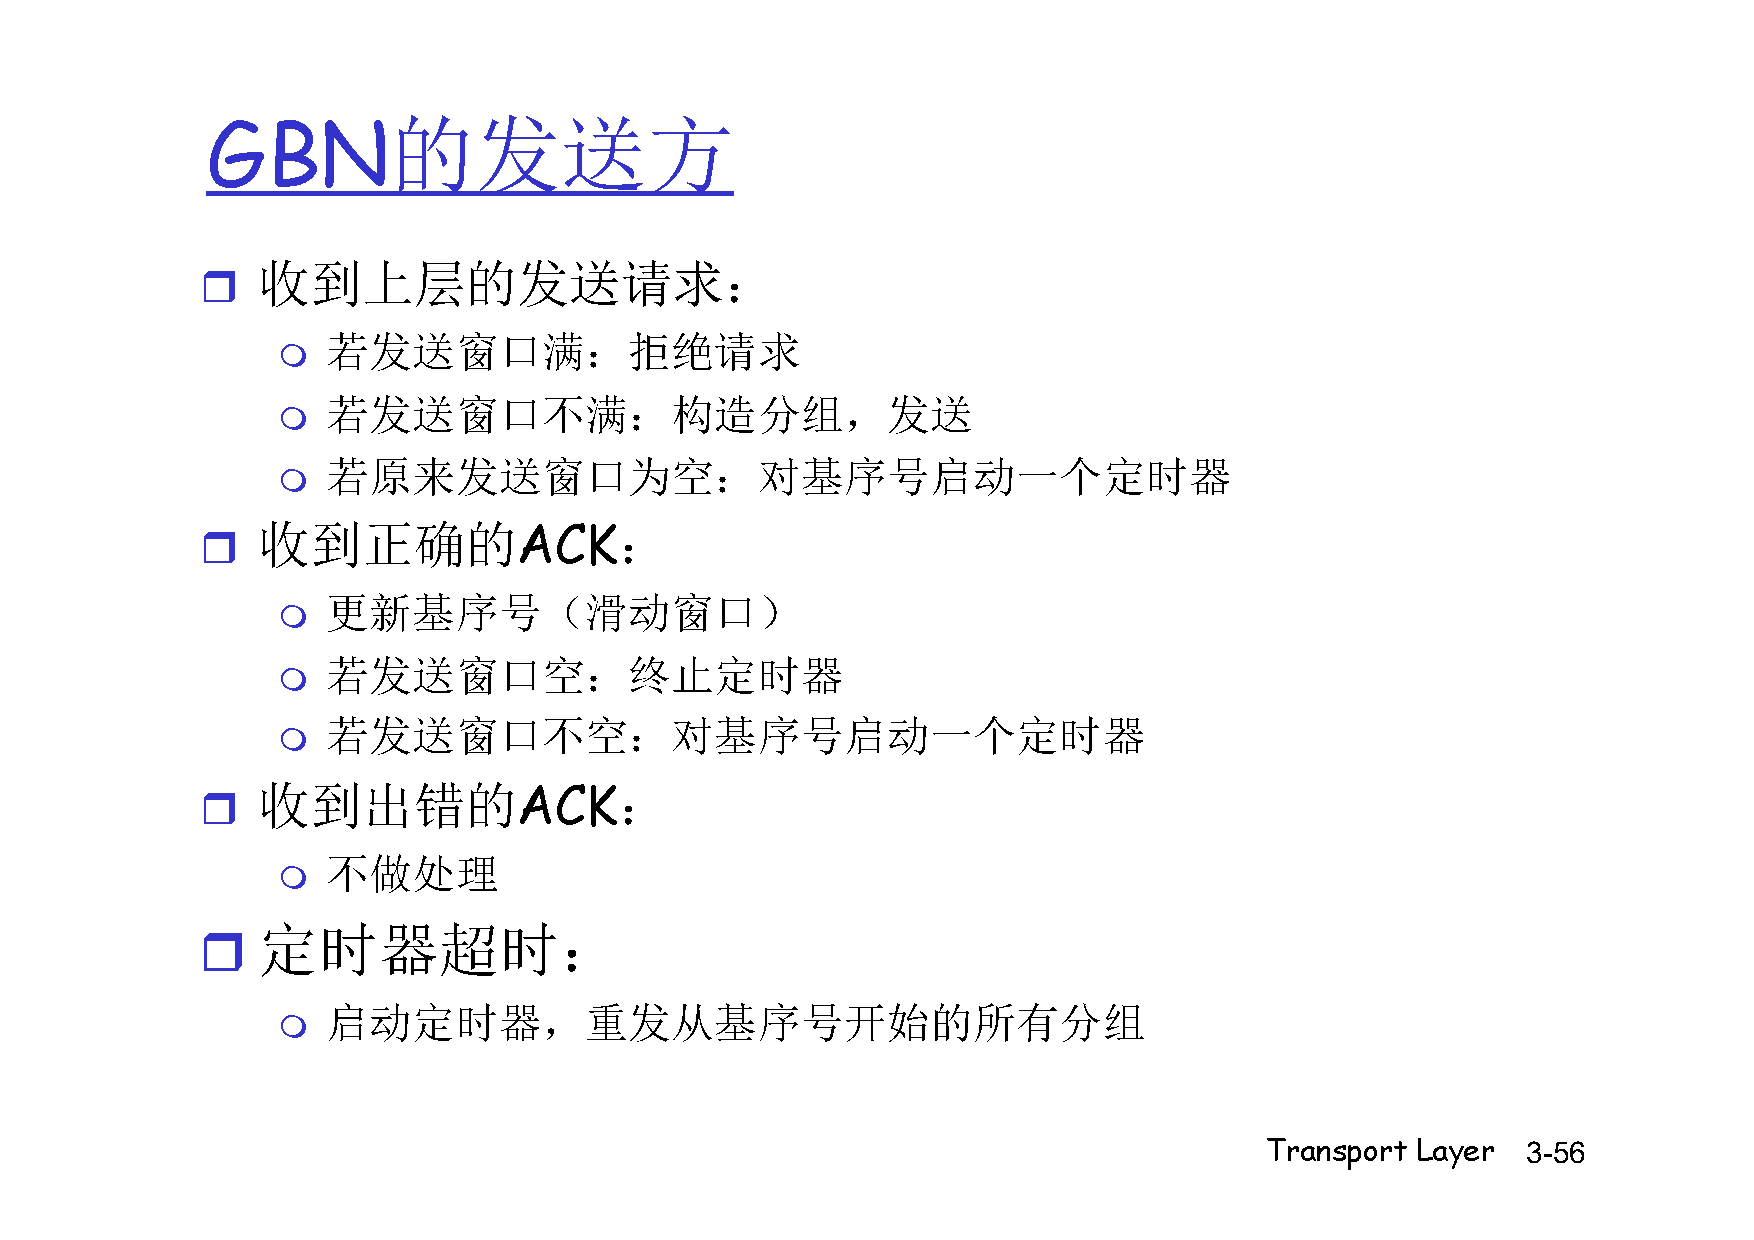
\includegraphics[scale = 0.35]{images/GBN_Sender_Time_Counter.pdf}
				\end{minipage}
			\end{figure}
		\subsection{选择重传}
			SR协议通过让发送方仅重传那些它怀疑在接收方出错(丢失或受损)的分组而避免了不必要的重传。
			SR协议与GBN有一些不同:因为SR的每一个分组都是独立的
			\begin{enumerate}
				\item 计时器:SR的每一个分组都要有自己的一个计时器,因为超时发生后只能发送一个分组
				\item 窗口移动:如果收到ACK是send\_base(窗口的第一个),窗口基序号移动到具有最小序号的未确认分组处
				\item 发送新的分组:(这两个都是)发送在窗口内且还没发出去的分组
				\item 收到ACK:标记这个分组为已接受
				\item 重复ACK:接收方在接收到窗口头之前的分组时,还是需要发送ACK,因为这个分组有可能时因为它的ACK没有成功到达发送方或者发送方超时,导致发送方重传,所以还是需要通知发送方
				\item 窗口大小:窗口长度必须小于等于序号空间的一半
			\end{enumerate}
	\section{面向连接的传输:TCP}
		TCP即传输控制协议,是因特网运输层的面向连接的可靠的运输协议。为了提供可靠数据传输,TCP依赖于前面提到的许多基本原理,包括差错检测、重传、累积确认、定时器以及用于序号和确认号的首部字段。\par
		总的来讲,TCP是一种较为“繁琐”的传输协议,双方需要相互握手,并采取很多措施,用时间来换取传输的正确性。TCP传输有如下特点:
		\begin{enumerate}
			\item 点到点通信:一个发送者,一个接收者
			\item 全双工:可以同时双向传输数据
			\item 面向连接:通信前双方先握手(交换控制报文),建立数据传输所需的状态(缓存、变量等)
			\item 可靠、有序的字节流:不保留报文(应用程序的输出)边界
			\item 流水式发送报文段:发送窗口由拥塞控制和流量控制机制设置
			\item 流量控制:发送方不会令接收方缓存溢出
		\end{enumerate}
		TCP可从缓存中取出并放入报文段中的数据量受限于最大报文段长度(MSS),它通常根据最初确定的由本地发送主机发送的最大链路层帧长度(即所谓的最大传输单元(MTU))来设置。注意MSS是指在报文段里\textbf{应用层数据}的最大长度,而不是包括首部的TCP报文段最大长度。建立连接时,每个主机可声明自己能够接受的MSS,缺省为536字节
		\subsection{段结构}
			TCP报文段由首部字段和一个数据字段组成。总的来看,TCP报文段为如下格式:\par
			\begin{figure}[h!]
				\centering
				\begin{minipage}{20em}
					\centering
					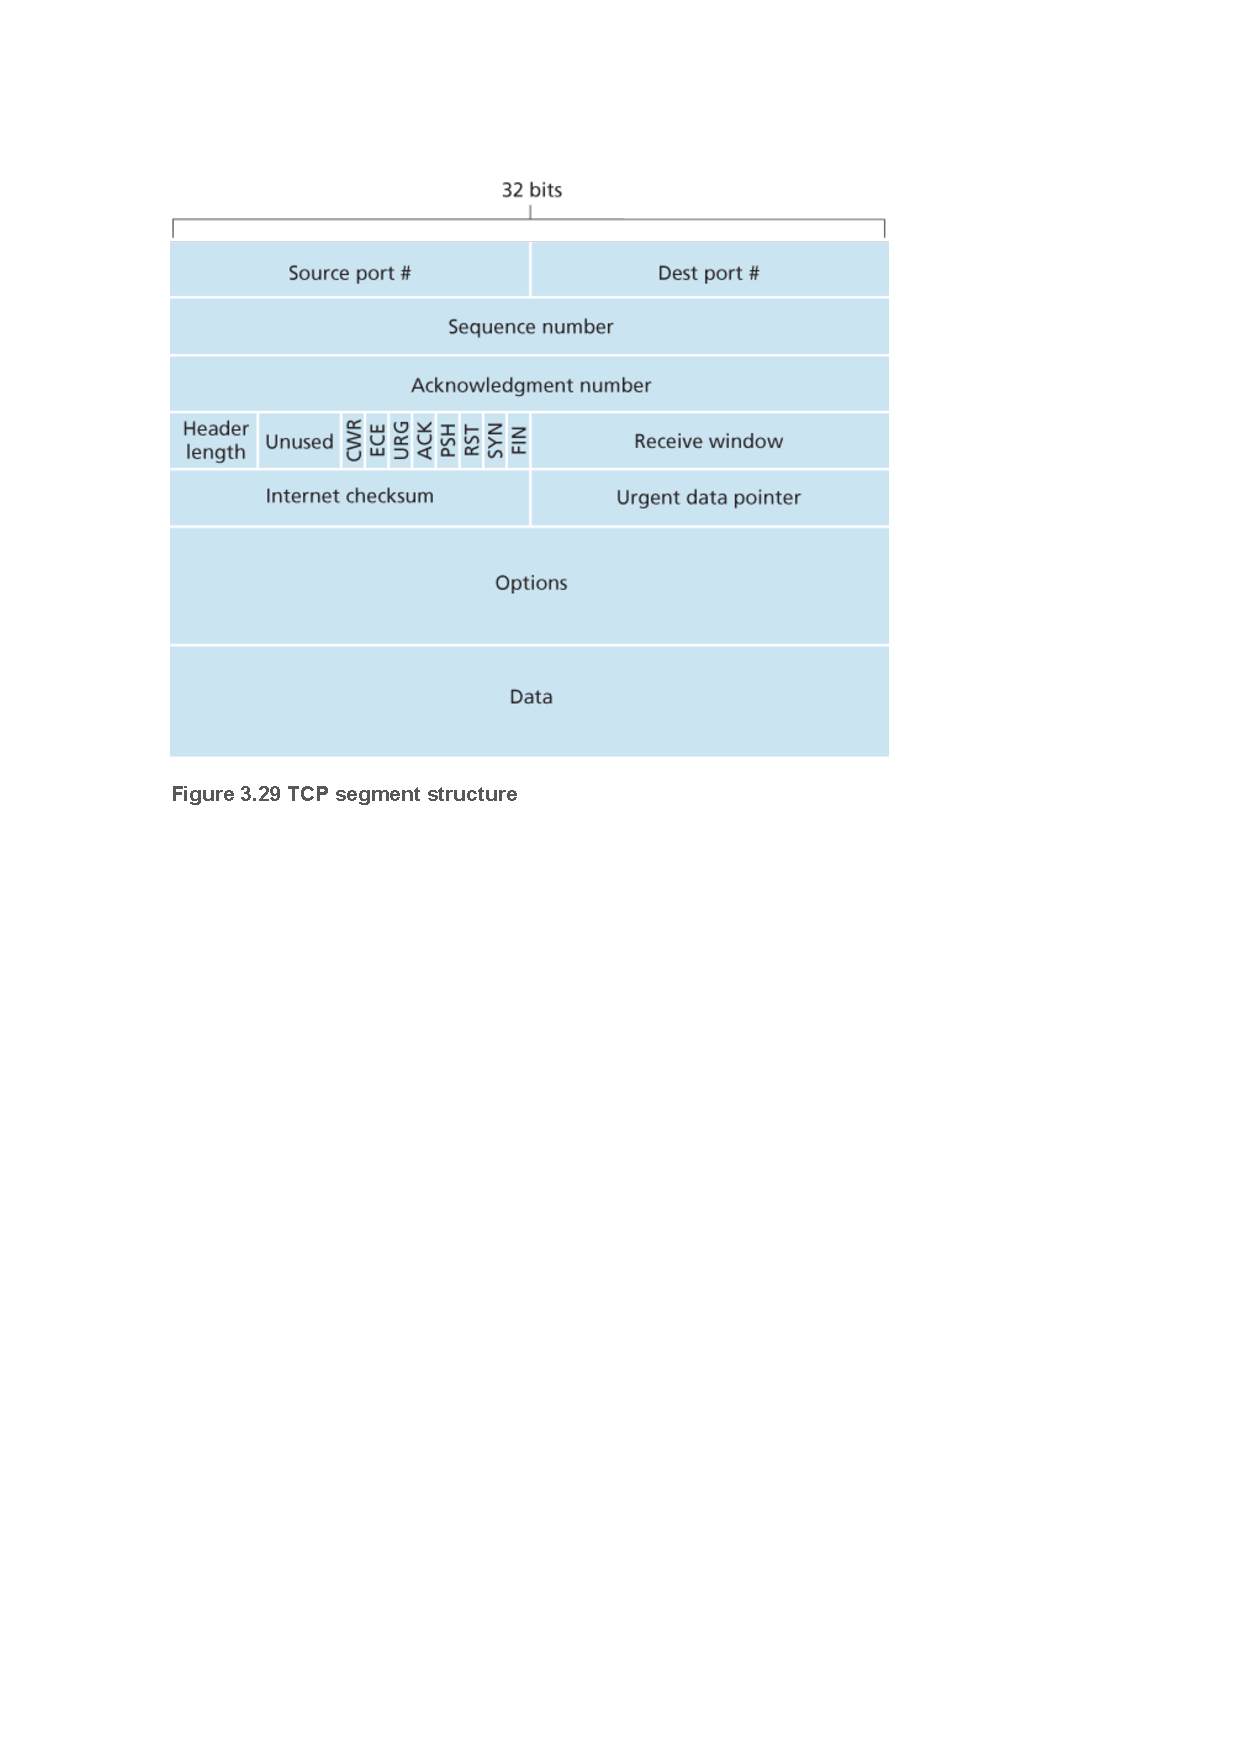
\includegraphics[scale = 0.5]{images/TCP_Segment_Structure.pdf}
				\end{minipage}
				\begin{minipage}{20em}
					\centering
					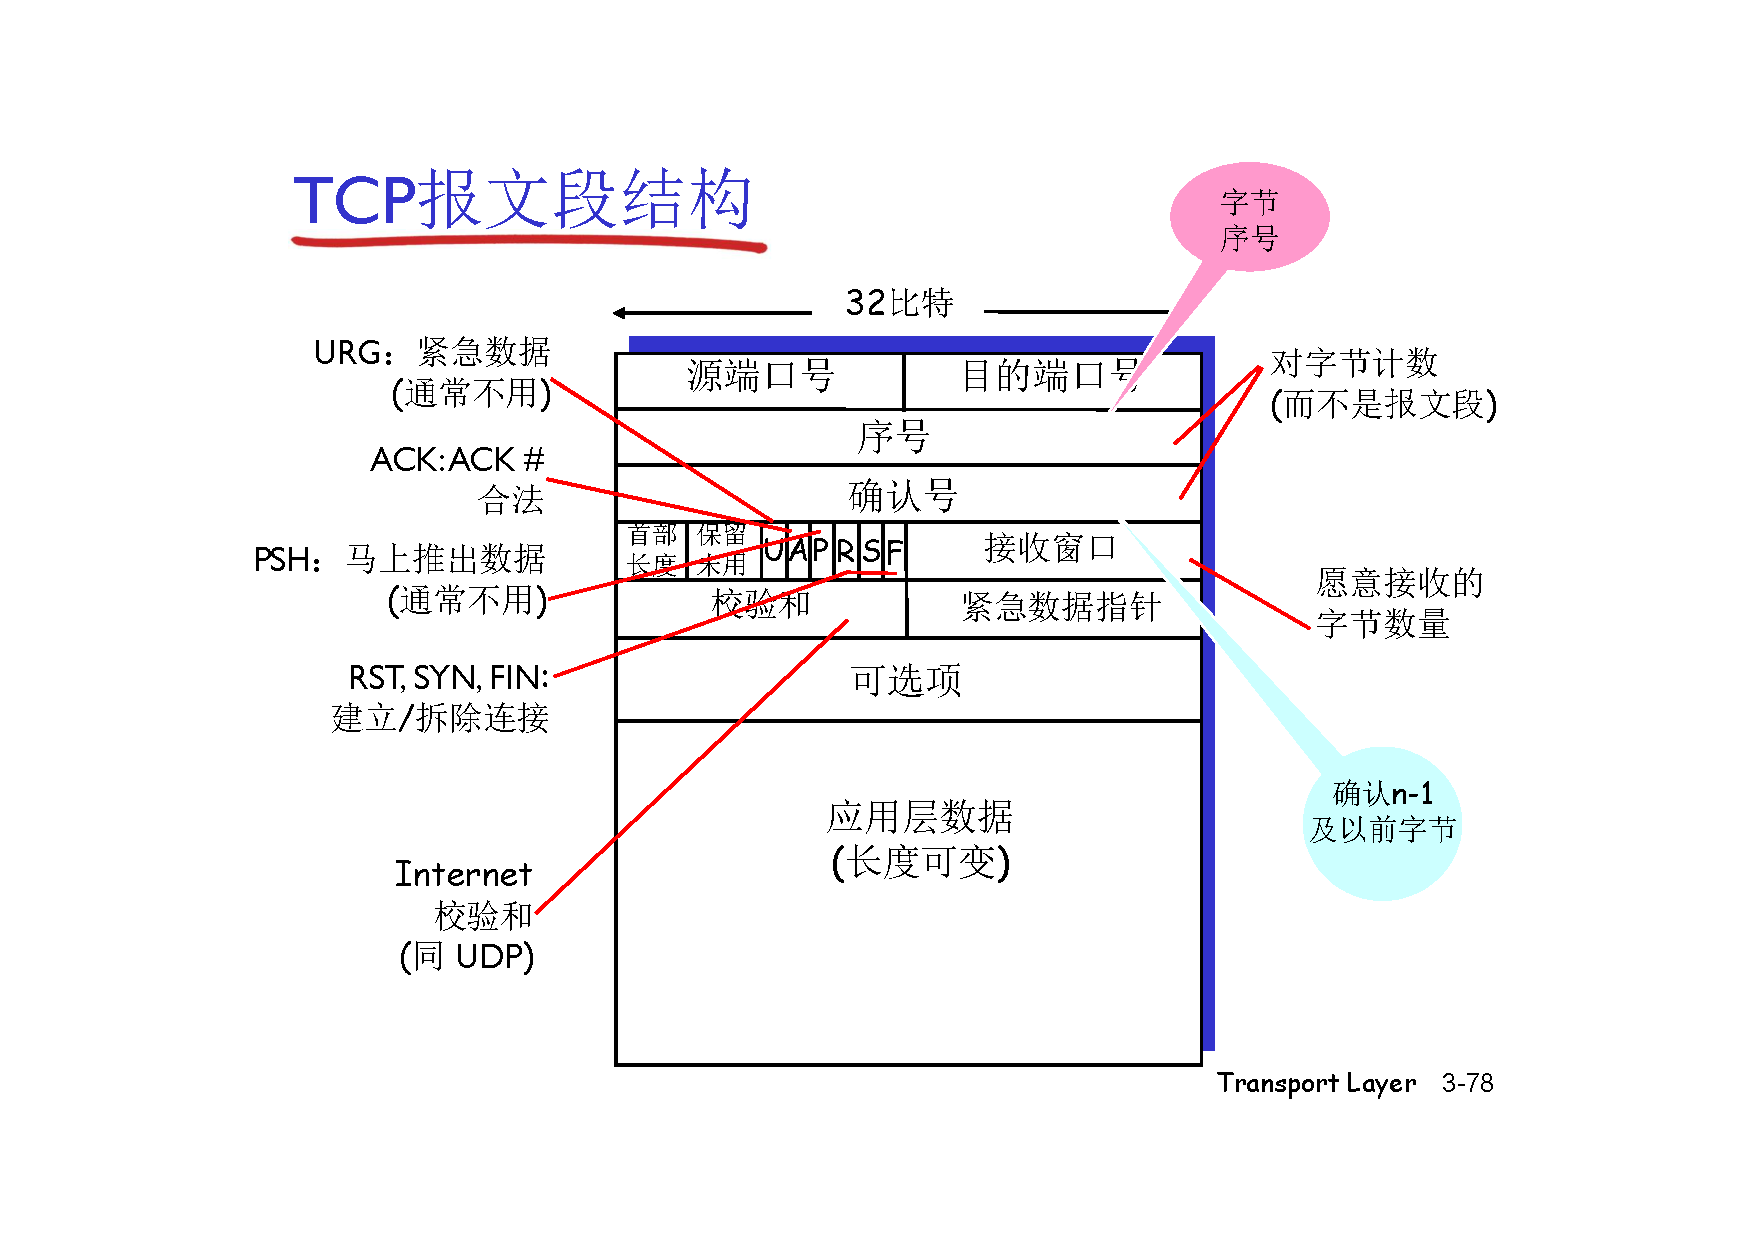
\includegraphics[scale = 0.3]{images/TCP_Segment_2nd.pdf}
				\end{minipage}
			\end{figure}
			对部分内容的解释如下:
			\begin{enumerate}
				\item 4bit的首部长度字段:由于TCP选项字段的原因,TCP首部的长度是可变的。
				\item 可选与变长的选项字段:用于发送方和接收方协商最大报文段长度MSS时,或在高速网络环境下用作窗口调节因子时使用
				\item 还定义了一个时间戳选项
			\end{enumerate}
			\paragraph{序号和确认号}
			TCP把数据看成是一个无结构的、有序的字节流。一个\textit{报文段}的序号是该报文段首字节的字节流编号。所以说相邻的报文段,其编号是不相邻的,间隔为MSS。对于确认号,接收方发送的确认号是\textit{期望}从发送方接到的下一\textbf{字节}的序号。TCP采用的是提供累积确认
		\subsection{可靠数据传输}
		\subsection{流量控制}
		\subsection{连接管理}
	\section{拥塞控制原理}
	\section{TCP拥塞控制}

	\chapter{网络层-数据平面}
	网络层是协议栈中最复杂的层次之一,因此我们将仔细考察两种用于构造网络层分组交换的方法,即数据报模式和虚电路模式,并且理解编址在传递分组到目的主机的重要作用。转发涉及在单一的路由器中从一条入链路到一条出链路到传送。路由选择涉及到一个网络的所有路由器,他们经路由选择协议共同交互,以决定目标分组从源到目的地结点所采用的路径。\textit{“虚电路和数据报网络”部分在第六版的书上,其余部分由第六版和第七版整理而成}\par
	因特网的网络层有三个主要组件: \circled{1}IP协议 \circled{2}路由选择部分(决定了数据报从源到目的地所经过的路径,会计算出用于在网络中转发分组的转发表) \circled{3}报告数据报中的差错和对某些网络层信息请求进行相应的设施

	\section{导论}
		网络层的关键功能:转发(通过单个路口的过程)和路由(从源到目的的路由规划路径过程)。
		\subsection{数据平面}
		\subsection{控制平面}
	\section{虚电路和数据报网络}
	与传输层提供的\textit{面向连接和无连接}服务相对应,网络层提供了\textit{连接和无连接}服务(注意这里不叫面向连接)。注意网络层和传输层服务之间的巨大差异:
	\begin{enumerate}
		\item 网络层向运输层提供主机到主机的服务,而运输层向应用层提供进程到进程的服务
		\item 在至今为止的所有的主要的计算机网络体系结构中(因特网、ATM、帧中继等),网络层提供且仅提供连接和无连接两种服务中的一种,而不同时提供两种服务。仅在网络层提供连接服务的计算机网络称为虚电路网络,仅在网络层提供无连接服务的计算机网络成为数据报网络
		\item 在运输层实现面向连接的服务和在网络层实现连接服务是完全不同的,运输层是在位于网络边缘的端系统中实现的,网络层也要在位于网络核心的路由器中实现。
	\end{enumerate}
		\subsection{虚电路网络}
		一条虚电路的组成如下:\circled{1}源和目的主机之间的路径(即一系列链路和路由器);\circled{2}VC号,沿着该路径的每段链路的一个号码;\circled{3}沿着该路径的每台路由器中的转发表表项。属于一条虚电路的分组将在它的首部携带一个VC号。因为一条虚电路在每条链路上可能具有不同的VC号,每台中间路由器必须用一个新的VC号替代每个传输分组的VC号。该新的VC号从转发表获得。\par
		换句话说,当一个分组离开端主机或者路由器时,会携带着一个VC号,当它途径(已经设定好的路径上的)路由器时,它的VC号会发生相应的改变,而改变规则是由转发表决定的。这么大一个网络,会有更多的路径组合,再加上路由器会有多个出入口,那会产生很多很多的表项更换关系。转发表又是怎么确定应该如何更改VC号的呢?有如下原理:无论何时跨越一台路由器创建一条新的虚电路,转发表就增加了一个新表项。类似地,无论何时终止一条虚电路,沿着该路径每个表中的相应项将被删除。\par
		那么,为什么还需要这个转换,而不是在每条链路上简单保持相同的VC号呢?第一,逐电路代替该号码减少了在分组首部中VC字段的长度。第二(but more importantly),可以大大简化虚电路的建立。{\color[HTML]{FF7F50}{特别是在具有多个VC号的路径,其上的每条链路要求……(第六版电子书P227中间)}}
		\subsection{数据报网络}
		在数据报网络中,一个端系统要发送分组,就为该分组加上目的端系统的地址,然后将分组推进网络中。在传播过程中,经过的每一台路由器都使用分组中的目标地址来转发该分组。特别是,每台路由器中有一个将\textbf{目的地址}映射到链路接口的转发表;当分组到达路由器时,路由器使用该分组的目的地址在转发表中查找适当的输出链路接口。\par
		数据报网络维护的转发表是由目的地址范围(由一个前缀匹配表示,它其实\textbf{可以}是另一个前缀匹配的前缀,在匹配时按照特殊优先的原则不会冲突,即\textit{最长前缀匹配规则})和对应的转发到的链路接口组成。\par
		虽然在数据报网络中的路由器不维持连接状态信息,但他们无论如何(whatever)在其转发表中维持了转发状态信息。
	\section{路由器组成}
	路由器由四个组件构成:路由选择处理器(在控制平面,软件)、输入端口、输出端口、交换结构(都是在数据平面、硬件)。
		\subsection{输入端口处理和基于目的地转发}
		输入端口的线路端接功能与链路层处理实现了用于各个输入链路的物理层和链路层。在输入端口中执行的查找对于路由器的运行是至关重要的。转发表是由路由选择处理器计算和更新的,但转发表的一份影子副本通常会被放在每个输入端口。{\color[HTML]{FF7F50}{使用在每个输入端口的影子副本,转发决策能在每个输入端口本地做出,无需基于每个分组调用集中式路由选择处理器,因此避免了集中式处理的瓶颈。}}尽管“查找”在输入端口处理中可认为是最为重要的动作,但必须采取许多其他动作:
		\begin{enumerate}[label = \circled{\arabic{*}}]
			\item 必须出现物理层和链路层处理
			\item 必须检查分组但版本号、检验和以及寿命字段,并且重写后两个字段
			\item 必须更新用于网络管理但计数器(如接收到的IP数据报的数目)
		\end{enumerate}
		所以输入端口步骤如下:线路端接 $\to$数据链路处理(协议,拆封)$\to$查找,转发,排队$\to$交换结构\par
		为了保证查找的效率,会用嵌入式片上DRAM和更快的SRAM(用作一种DRAM缓存)内存来设计。三态内容可寻址存储器也常被用于查找
		\subsection{交换结构}
		交换节点位于一台路由器的核心部位。有三种交换技术:
			\paragraph{经内存交换}
			最简单、最早的路由器是传统的计算机,在输入端口与输出端口之间的交换是在CPU(路由选择处理器)的直接控制下完成的。输入和输出端口的功能就像在传统操作系统中的I/O设备一样。许多现代路由器(尤其适合小容量路由器)用内存进行交换,但目的地址但查找和将分组存储(交换)进适当的内存 存储位置是由输入线路卡来处理的
			\paragraph{经总线交换}
			让输入端口为分组预先计划一个交换机内部标签(首部),指示本地输出端口。该分组能由所有输出端口收到,但只有与该便签匹配的端口才能保存该分组。然后标签在输出端口被去除,因为其仅用于交换机内部来跨越总线。因为每个分组必须跨越单一总线,故路由器的交换带宽受总线速率的限制。对于运行在小型局域网和企业网中的路由器来说,通过总线交换通常是足够的。
			\paragraph{经互联网络交换}
			克服单一、共享式带宽限制的一种方法是,使用一个更复杂的互联网络。纵横式交换机就是一种由2N条总线组成的互联网络,它连接N个输入端口与N个输出端口(如下图),交叉结点可以选择打开和闭合。
			\begin{figure}
				\centering
				\begin{minipage}{40em}
					\centering
					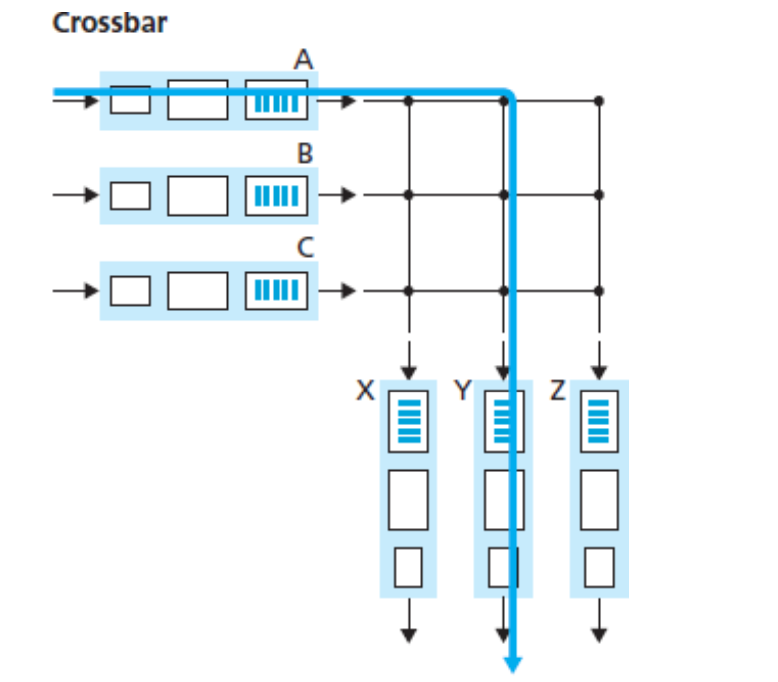
\includegraphics[scale = 0.5]{images/crossbar_in_router.png}
				\end{minipage}
			\end{figure}\par
			与前面两种交换方式不同,纵横式网络能够并行转发多个分组。纵横式交换机是\textbf{非阻塞的},即只要没有其他分组被转发到该输入端口,转发到输出端口的分组将不会被到达输出端口的分组阻塞。但如果来自两个不同输入端口的分组,则某个时间经给定总线仅能够发送一个分组
		\subsection{输出端口}
		交换结构$\to$排队(缓存管理)$\to$数据链路处理(协议、封装)$\to$线路端接
		\subsection{何处出现排队}
		显然在输入端口和输出端口都会形成排队,这些队列占用了路由器的缓存空间,当缓冲区满时将会产生丢包。在下面的讨论中,设输入链路速率和输出链路速率均为$R_{line}$,且有N个输入端口和N个输出端口。定义交换结构传送速率$R_{switch}$为从输入端口到输出端口能够移动分组的速率。速率的单位均为(分组/秒)
			\paragraph{输入排队}
			和交换结构传送速率与输入速率有关。考虑纵横式结构,并做如下假定:
			\begin{enumerate}
				\item 所有链路速度相同
				\item 一个分组能够以一条输入链路接受一个分组所用的相同的时间量,从任意一个输出端口传送到给定的输出端口(也就是说,去除排队的时间,分组经过输入部分和经过交换结构的时间相同)
				\item 分组在输入队列是FCFS的,在交换结构中只要输出端口不同就是并行的,否则除其中一个外会被阻塞
			\end{enumerate}
			会出现如下情况:假设输入端口A和B头部的两个分组1和2都要发往接受端口a,不妨假设交换结构决定发送分组1.那么这个时候,即使分组2后面的分组3是发往端口b(并无竞争),它也需要等待。这种现象称为输入排队交换机中的线路前部(HOL)阻塞。由于HOL阻塞,只要输入链路上的分组到达速率达到其容量的58\%,在某些假设前提下,输入队列的长度就将无限制增大。
			\paragraph{输出排队}
			输出端口的排队和输出端口发送分组的速率与交换结构的传送速率有关。假设$R_{switch}=N\times R_{line}$,这时候输入端口不会产生排队,但是输出端口很有可能排队。\par
			当缓冲区满的时候,要么丢弃到达的分组(弃尾),要么删除一个或多个以排队的分组。在某些情况下,在缓存填满之前就丢弃一个分组(或在其首部加上标记)的做法是有利的,这可以向发送方提供一个拥塞信号。这些分组丢弃和标记策略统称为主动队列管理(AQM)
			\paragraph{路由器缓存}
			假定需要路由器缓存来吸收流量负载的波动。多年以来,用于缓存长度的经验方法是[RFC 3439],缓存数量B等于平均往返时延RTT乘以链路的容量C。这个结果是对于少量TCP流的排队动态性分析得到的。当有大量的TCP流(如N条)流过一条链路时,缓存所需要的数量是$B=RTT\times C/\sqrt{N}$
		\subsection{分组调度}
		现在讨论确定次序的问题,即\textit{排队的分组如何经输出链路传输}的问题。这块参考OS的进程调度,三种策略分别是FIFO、priority和RR
			\paragraph{先进先出}
			如果没有足够的缓存空间来容纳到达的分组,队列的分组丢弃策略则确定该分组是否将被丢弃(丢失)或者从队列中去除其他分组以便为到达的分组腾出空间。
			\paragraph{优先权排队}
			在实践中,网络操作员可以配置一个队列,这样携带网络管理信息的分组(例如,由源或目的TCP/UDP端口号所标示)获得超过用户流量的优先权;此外,基于IP的实时话音分组可能获得超过非实时流量的优先权。\par
			在非抢占式优先权排队规则下,一旦分组开始传输,就不能打断。
			\paragraph{循环和加权公平排队}
			在循环排队规则下,分组像使用优先权排队那样被分类。但是是采用Round-Robin的方式来发送各个类的分组。一个所谓的保持工作排队规则是在有(任何类的)分组等待传输时,不允许链路保持空闲。当寻找给定的类的分组但没有找到时,保持工作的循环规则将立即检查循环序列中的下一个类。\par
			加权公平排队(WFQ)规则中,到达的分组被分类并在合适的等待区域排队,同样采用Round-Robin的方式来对各个类进行轮转。WFQ和循环排队的不同之处在于,每个类在任何时间间隔内可能收到不同数量的服务。具体而言,每个类被分配一个权$w_i$。使用WFQ方式,在类i有分组要发送的任何时间间隔中,第i类将确保接收到的服务部分等于$w_i/(\sum w_j)$部分。
	\section{网际协议:IPv4、寻址、IPv6及其他}
	在这节中,我们将关注点转向今天的因特网网络层的关键方面和著名的网际协议(IP)。今天有两个版本的IP正使用:IP版本4(IPv4)和IPv6
		\subsection{数据报格式}
		IPv4中的关键字段(部分)如下:
		\begin{enumerate}
			\item 服务类型(TOS)区分不同类型的数据报(如,以下特别要求低时延、高吞吐量或可靠性的数据报)
			\item 标识、标志、片偏移与IP分片有关。IPv6不允许在路由器上对分组分片
			\item 寿命(TTL)
			\item 协议通常仅当到达最终目的地才有用。指示了其数据部分应当交给哪个特定的运输层协议。如:值为6是TCP,值为17是UDP。注意在IP数据报中对协议号所起的作用,类似于运输层报文段中端口号字段所起的作用
			\item 首部检验和与该和的反码(被称为因特网检验和)存放在检验和字段中。注意在每台路由器上必须\textbf{重新计算}检验和并再次存放到原处,因为TTL字段及可能的选项字段会改变。\textit{为什么TCP/TP在运输层和网络层都执行差错检测?}首先,IP只对IP首部计算了检验和,而TCP/UDP检验是对整个TCP/UDP报文段进行的;其次,TCP/UDP和IP不一定属于同一个协议栈
		\end{enumerate}
		\subsection{分片}
		\subsection{Ipv4地址}
		\subsection{NAT:网络地址转换}
		\subsection{Ipv6}
	\section{通用转发和SDN}
		\subsection{匹配}
		\subsection{行动}
		\subsection{OpenFLow有关“匹配+行动”的运行实例}
\end{document}
